\documentclass[a4paper]{book}
\usepackage{a4wide}
\usepackage{makeidx}
\usepackage{fancyhdr}
\usepackage{graphicx}
\usepackage{multicol}
\usepackage{float}
\usepackage{textcomp}
\usepackage{alltt}
\usepackage{times}
\usepackage{ifpdf}
\ifpdf
\usepackage[pdftex,
            pagebackref=true,
            colorlinks=true,
            linkcolor=blue,
            unicode
           ]{hyperref}
\else
\usepackage[ps2pdf,
            pagebackref=true,
            colorlinks=true,
            linkcolor=blue,
            unicode
           ]{hyperref}
\usepackage{pspicture}
\fi
\usepackage[utf8]{inputenc}
\usepackage{doxygen}
\makeindex
\setcounter{tocdepth}{1}
\renewcommand{\footrulewidth}{0.4pt}
\begin{document}
\begin{titlepage}
\vspace*{7cm}
\begin{center}
{\Large ACO-R \\[1ex]\large 1 }\\
\vspace*{1cm}
{\large Generated by Doxygen 1.5.5}\\
\vspace*{0.5cm}
{\small Wed Feb 4 11:12:19 2009}\\
\end{center}
\end{titlepage}
\clearemptydoublepage
\pagenumbering{roman}
\tableofcontents
\clearemptydoublepage
\pagenumbering{arabic}
\chapter{Class Index}
\section{Class Hierarchy}
This inheritance list is sorted roughly, but not completely, alphabetically:\begin{CompactList}
\item \contentsline{section}{Colony}{\pageref{classColony}}{}
\item \contentsline{section}{Function}{\pageref{classFunction}}{}
\begin{CompactList}
\item \contentsline{section}{Ackley}{\pageref{classAckley}}{}
\item \contentsline{section}{Griewank}{\pageref{classGriewank}}{}
\item \contentsline{section}{Rastrigin}{\pageref{classRastrigin}}{}
\end{CompactList}
\item \contentsline{section}{Random}{\pageref{classRandom}}{}
\item \contentsline{section}{Solution}{\pageref{classSolution}}{}
\item \contentsline{section}{Timer}{\pageref{classTimer}}{}
\end{CompactList}

\chapter{Class Index}
\section{Class List}
Here are the classes, structs, unions and interfaces with brief descriptions:\begin{CompactList}
\item\contentsline{section}{\hyperlink{classAckley}{Ackley} }{\pageref{classAckley}}{}
\item\contentsline{section}{\hyperlink{classColony}{Colony} }{\pageref{classColony}}{}
\item\contentsline{section}{\hyperlink{classFunction}{Function} }{\pageref{classFunction}}{}
\item\contentsline{section}{\hyperlink{classGriewank}{Griewank} }{\pageref{classGriewank}}{}
\item\contentsline{section}{\hyperlink{classRandom}{Random} }{\pageref{classRandom}}{}
\item\contentsline{section}{\hyperlink{classRastrigin}{Rastrigin} }{\pageref{classRastrigin}}{}
\item\contentsline{section}{\hyperlink{classSolution}{Solution} }{\pageref{classSolution}}{}
\item\contentsline{section}{\hyperlink{classTimer}{Timer} }{\pageref{classTimer}}{}
\end{CompactList}

\chapter{File Index}
\section{File List}
Here is a list of all files with brief descriptions:\begin{CompactList}
\item\contentsline{section}{/home/andrej/workspace/hpso/pso\_\-src/\hyperlink{1run__pso_8py}{1run\_\-pso.py} }{\pageref{1run__pso_8py}}{}
\item\contentsline{section}{/home/andrej/workspace/hpso/pso\_\-src/\hyperlink{1writeBatch_8py}{1writeBatch.py} }{\pageref{1writeBatch_8py}}{}
\item\contentsline{section}{/home/andrej/workspace/hpso/pso\_\-src/\hyperlink{bird_8cpp}{bird.cpp} }{\pageref{bird_8cpp}}{}
\item\contentsline{section}{/home/andrej/workspace/hpso/pso\_\-src/\hyperlink{bird_8h}{bird.h} }{\pageref{bird_8h}}{}
\item\contentsline{section}{/home/andrej/workspace/hpso/pso\_\-src/\hyperlink{displayGraph_8py}{displayGraph.py} }{\pageref{displayGraph_8py}}{}
\item\contentsline{section}{/home/andrej/workspace/hpso/pso\_\-src/\hyperlink{lsearch_8cpp}{lsearch.cpp} }{\pageref{lsearch_8cpp}}{}
\item\contentsline{section}{/home/andrej/workspace/hpso/pso\_\-src/\hyperlink{lsearch_8h}{lsearch.h} }{\pageref{lsearch_8h}}{}
\item\contentsline{section}{/home/andrej/workspace/hpso/pso\_\-src/\hyperlink{movpeaks_8c}{movpeaks.c} }{\pageref{movpeaks_8c}}{}
\item\contentsline{section}{/home/andrej/workspace/hpso/pso\_\-src/\hyperlink{movpeaks_8h}{movpeaks.h} }{\pageref{movpeaks_8h}}{}
\item\contentsline{section}{/home/andrej/workspace/hpso/pso\_\-src/\hyperlink{optfunctions_8cpp}{optfunctions.cpp} }{\pageref{optfunctions_8cpp}}{}
\item\contentsline{section}{/home/andrej/workspace/hpso/pso\_\-src/\hyperlink{optfunctions_8h}{optfunctions.h} }{\pageref{optfunctions_8h}}{}
\item\contentsline{section}{/home/andrej/workspace/hpso/pso\_\-src/\hyperlink{optimumrun_8py}{optimumrun.py} }{\pageref{optimumrun_8py}}{}
\item\contentsline{section}{/home/andrej/workspace/hpso/pso\_\-src/\hyperlink{paramWindow_8py}{paramWindow.py} }{\pageref{paramWindow_8py}}{}
\item\contentsline{section}{/home/andrej/workspace/hpso/pso\_\-src/\hyperlink{pso_8cpp}{pso.cpp} }{\pageref{pso_8cpp}}{}
\item\contentsline{section}{/home/andrej/workspace/hpso/pso\_\-src/\hyperlink{pso_8h}{pso.h} }{\pageref{pso_8h}}{}
\item\contentsline{section}{/home/andrej/workspace/hpso/pso\_\-src/\hyperlink{pso_8py}{pso.py} }{\pageref{pso_8py}}{}
\item\contentsline{section}{/home/andrej/workspace/hpso/pso\_\-src/\hyperlink{pso__globals_8cpp}{pso\_\-globals.cpp} }{\pageref{pso__globals_8cpp}}{}
\item\contentsline{section}{/home/andrej/workspace/hpso/pso\_\-src/\hyperlink{pso__globals_8h}{pso\_\-globals.h} }{\pageref{pso__globals_8h}}{}
\item\contentsline{section}{/home/andrej/workspace/hpso/pso\_\-src/\hyperlink{pso__statistics_8cpp}{pso\_\-statistics.cpp} }{\pageref{pso__statistics_8cpp}}{}
\item\contentsline{section}{/home/andrej/workspace/hpso/pso\_\-src/\hyperlink{pso__statistics_8h}{pso\_\-statistics.h} }{\pageref{pso__statistics_8h}}{}
\item\contentsline{section}{/home/andrej/workspace/hpso/pso\_\-src/\hyperlink{pso__wrap_8cpp}{pso\_\-wrap.cpp} }{\pageref{pso__wrap_8cpp}}{}
\item\contentsline{section}{/home/andrej/workspace/hpso/pso\_\-src/\hyperlink{psoParameter-old_8py}{psoParameter-old.py} }{\pageref{psoParameter-old_8py}}{}
\item\contentsline{section}{/home/andrej/workspace/hpso/pso\_\-src/\hyperlink{psoParameter_8py}{psoParameter.py} }{\pageref{psoParameter_8py}}{}
\item\contentsline{section}{/home/andrej/workspace/hpso/pso\_\-src/\hyperlink{psostart_8py}{psostart.py} }{\pageref{psostart_8py}}{}
\item\contentsline{section}{/home/andrej/workspace/hpso/pso\_\-src/\hyperlink{run__pso_8py}{run\_\-pso.py} }{\pageref{run__pso_8py}}{}
\item\contentsline{section}{/home/andrej/workspace/hpso/pso\_\-src/\hyperlink{runpso_8cpp}{runpso.cpp} }{\pageref{runpso_8cpp}}{}
\item\contentsline{section}{/home/andrej/workspace/hpso/pso\_\-src/\hyperlink{showParameter_8py}{showParameter.py} }{\pageref{showParameter_8py}}{}
\item\contentsline{section}{/home/andrej/workspace/hpso/pso\_\-src/\hyperlink{swarm_8cpp}{swarm.cpp} }{\pageref{swarm_8cpp}}{}
\item\contentsline{section}{/home/andrej/workspace/hpso/pso\_\-src/\hyperlink{swarm_8h}{swarm.h} }{\pageref{swarm_8h}}{}
\item\contentsline{section}{/home/andrej/workspace/hpso/pso\_\-src/\hyperlink{test_8cpp}{test.cpp} }{\pageref{test_8cpp}}{}
\item\contentsline{section}{/home/andrej/workspace/hpso/pso\_\-src/\hyperlink{tools_8cpp}{tools.cpp} }{\pageref{tools_8cpp}}{}
\item\contentsline{section}{/home/andrej/workspace/hpso/pso\_\-src/\hyperlink{tools_8h}{tools.h} }{\pageref{tools_8h}}{}
\item\contentsline{section}{/home/andrej/workspace/hpso/pso\_\-src/\hyperlink{tree_8hh}{tree.hh} }{\pageref{tree_8hh}}{}
\item\contentsline{section}{/home/andrej/workspace/hpso/pso\_\-src/\hyperlink{writeBatch_8py}{writeBatch.py} }{\pageref{writeBatch_8py}}{}
\end{CompactList}

\chapter{Class Documentation}
\hypertarget{classAckley}{
\section{Ackley Class Reference}
\label{classAckley}\index{Ackley@{Ackley}}
}
{\tt \#include $<$Functions.h$>$}

Inheritance diagram for Ackley:\nopagebreak
\begin{figure}[H]
\begin{center}
\leavevmode
\includegraphics[width=49pt]{classAckley__inherit__graph}
\end{center}
\end{figure}
Collaboration diagram for Ackley:\nopagebreak
\begin{figure}[H]
\begin{center}
\leavevmode
\includegraphics[width=49pt]{classAckley__coll__graph}
\end{center}
\end{figure}
\subsection*{Public Member Functions}
\begin{CompactItemize}
\item 
\hyperlink{classAckley_6f846d6b110026aa8f6d59ce7f1caf9a}{Ackley} (int \hyperlink{aco-r_8cpp_1a8a8235879363159315091a1daed72f}{dimension}=10)
\item 
virtual double \hyperlink{classAckley_6423fcd54b72322f08357879bac580b6}{evaluate} (vector$<$ double $>$ \&x)
\end{CompactItemize}


\subsection{Constructor \& Destructor Documentation}
\hypertarget{classAckley_6f846d6b110026aa8f6d59ce7f1caf9a}{
\index{Ackley@{Ackley}!Ackley@{Ackley}}
\index{Ackley@{Ackley}!Ackley@{Ackley}}
\subsubsection{\setlength{\rightskip}{0pt plus 5cm}Ackley::Ackley (int {\em dimension} = {\tt 10})}}
\label{classAckley_6f846d6b110026aa8f6d59ce7f1caf9a}




\subsection{Member Function Documentation}
\hypertarget{classAckley_6423fcd54b72322f08357879bac580b6}{
\index{Ackley@{Ackley}!evaluate@{evaluate}}
\index{evaluate@{evaluate}!Ackley@{Ackley}}
\subsubsection{\setlength{\rightskip}{0pt plus 5cm}double Ackley::evaluate (vector$<$ double $>$ \& {\em x})\hspace{0.3cm}{\tt  \mbox{[}virtual\mbox{]}}}}
\label{classAckley_6423fcd54b72322f08357879bac580b6}




Implements \hyperlink{classFunction_9323a7309b16e0e168590e34b359ff32}{Function}.

The documentation for this class was generated from the following files:\begin{CompactItemize}
\item 
\hyperlink{Functions_8h}{Functions.h}\item 
\hyperlink{Functions_8cpp}{Functions.cpp}\end{CompactItemize}

\hypertarget{classColony}{
\section{Colony Class Reference}
\label{classColony}\index{Colony@{Colony}}
}
{\tt \#include $<$Colony.h$>$}

Collaboration diagram for Colony:\nopagebreak
\begin{figure}[H]
\begin{center}
\leavevmode
\includegraphics[width=83pt]{classColony__coll__graph}
\end{center}
\end{figure}
\subsection*{Public Member Functions}
\begin{CompactItemize}
\item 
\hyperlink{classColony_af760edad97dee7263b86913d3bb4f98}{Colony} ()
\item 
\hyperlink{classColony_13871283edd253b794363e33a8920f6b}{Colony} (\hyperlink{classFunction}{Function} $\ast$my\_\-f, int my\_\-archive\_\-size, int my\_\-n\_\-of\_\-ants, double my\_\-q, double my\_\-rho)
\item 
\hyperlink{classColony_9cebe4a25260c8da7c99d10b0dab5a4e}{$\sim$Colony} ()
\item 
int \hyperlink{classColony_c46a39e897255d72662ed9b1677bc91a}{initialize} ()
\item 
int \hyperlink{classColony_81a0f7680e31680188f40f5293510711}{iterate} ()
\item 
void \hyperlink{classColony_ca86ca3a2dcad9f2e98edfb449c6bbe2}{delete\_\-worst} ()
\item 
double \hyperlink{classColony_392a128abc861f658f92aa98f6c21585}{gaussian} (double mean, double var)
\end{CompactItemize}
\subsection*{Public Attributes}
\begin{CompactItemize}
\item 
\hyperlink{classFunction}{Function} $\ast$ \hyperlink{classColony_bf5614747e9e944cd2af6ffa83e3cf38}{f}
\item 
\hyperlink{classSolution}{Solution} $\ast$ \hyperlink{classColony_3030d0a11898b83414df4a3f8878c141}{bestSol}
\item 
int \hyperlink{classColony_6ab1bba15c25d8c2e38e2a3632d63661}{archive\_\-size}
\item 
int \hyperlink{classColony_5398847209293075291ecec0c242b19e}{n\_\-of\_\-ants}
\item 
double \hyperlink{classColony_34885da4424133c87e8c887ea9b26f14}{q}
\item 
double \hyperlink{classColony_49231f75985e7ba471f22438e5449714}{rho}
\item 
list$<$ \hyperlink{classSolution}{Solution} $\ast$ $>$ \hyperlink{classColony_74323b8c562a6e02b786be593a6ad25b}{archive}
\item 
int \hyperlink{classColony_f6d58daa2f800a0c086c43ff0a8d49d0}{nonimpr\_\-counter}
\end{CompactItemize}


\subsection{Constructor \& Destructor Documentation}
\hypertarget{classColony_af760edad97dee7263b86913d3bb4f98}{
\index{Colony@{Colony}!Colony@{Colony}}
\index{Colony@{Colony}!Colony@{Colony}}
\subsubsection{\setlength{\rightskip}{0pt plus 5cm}Colony::Colony ()}}
\label{classColony_af760edad97dee7263b86913d3bb4f98}


\hypertarget{classColony_13871283edd253b794363e33a8920f6b}{
\index{Colony@{Colony}!Colony@{Colony}}
\index{Colony@{Colony}!Colony@{Colony}}
\subsubsection{\setlength{\rightskip}{0pt plus 5cm}Colony::Colony ({\bf Function} $\ast$ {\em my\_\-f}, \/  int {\em my\_\-archive\_\-size}, \/  int {\em my\_\-n\_\-of\_\-ants}, \/  double {\em my\_\-q}, \/  double {\em my\_\-rho})}}
\label{classColony_13871283edd253b794363e33a8920f6b}


\hypertarget{classColony_9cebe4a25260c8da7c99d10b0dab5a4e}{
\index{Colony@{Colony}!$\sim$Colony@{$\sim$Colony}}
\index{$\sim$Colony@{$\sim$Colony}!Colony@{Colony}}
\subsubsection{\setlength{\rightskip}{0pt plus 5cm}Colony::$\sim$Colony ()}}
\label{classColony_9cebe4a25260c8da7c99d10b0dab5a4e}




\subsection{Member Function Documentation}
\hypertarget{classColony_c46a39e897255d72662ed9b1677bc91a}{
\index{Colony@{Colony}!initialize@{initialize}}
\index{initialize@{initialize}!Colony@{Colony}}
\subsubsection{\setlength{\rightskip}{0pt plus 5cm}int Colony::initialize ()}}
\label{classColony_c46a39e897255d72662ed9b1677bc91a}




Here is the call graph for this function:\nopagebreak
\begin{figure}[H]
\begin{center}
\leavevmode
\includegraphics[width=132pt]{classColony_c46a39e897255d72662ed9b1677bc91a_cgraph}
\end{center}
\end{figure}
\hypertarget{classColony_81a0f7680e31680188f40f5293510711}{
\index{Colony@{Colony}!iterate@{iterate}}
\index{iterate@{iterate}!Colony@{Colony}}
\subsubsection{\setlength{\rightskip}{0pt plus 5cm}int Colony::iterate ()}}
\label{classColony_81a0f7680e31680188f40f5293510711}




Here is the call graph for this function:\nopagebreak
\begin{figure}[H]
\begin{center}
\leavevmode
\includegraphics[width=128pt]{classColony_81a0f7680e31680188f40f5293510711_cgraph}
\end{center}
\end{figure}
\hypertarget{classColony_ca86ca3a2dcad9f2e98edfb449c6bbe2}{
\index{Colony@{Colony}!delete\_\-worst@{delete\_\-worst}}
\index{delete\_\-worst@{delete\_\-worst}!Colony@{Colony}}
\subsubsection{\setlength{\rightskip}{0pt plus 5cm}void Colony::delete\_\-worst ()}}
\label{classColony_ca86ca3a2dcad9f2e98edfb449c6bbe2}


\hypertarget{classColony_392a128abc861f658f92aa98f6c21585}{
\index{Colony@{Colony}!gaussian@{gaussian}}
\index{gaussian@{gaussian}!Colony@{Colony}}
\subsubsection{\setlength{\rightskip}{0pt plus 5cm}double Colony::gaussian (double {\em mean}, \/  double {\em var})}}
\label{classColony_392a128abc861f658f92aa98f6c21585}




\subsection{Member Data Documentation}
\hypertarget{classColony_bf5614747e9e944cd2af6ffa83e3cf38}{
\index{Colony@{Colony}!f@{f}}
\index{f@{f}!Colony@{Colony}}
\subsubsection{\setlength{\rightskip}{0pt plus 5cm}{\bf Function}$\ast$ {\bf Colony::f}}}
\label{classColony_bf5614747e9e944cd2af6ffa83e3cf38}


\hypertarget{classColony_3030d0a11898b83414df4a3f8878c141}{
\index{Colony@{Colony}!bestSol@{bestSol}}
\index{bestSol@{bestSol}!Colony@{Colony}}
\subsubsection{\setlength{\rightskip}{0pt plus 5cm}{\bf Solution}$\ast$ {\bf Colony::bestSol}}}
\label{classColony_3030d0a11898b83414df4a3f8878c141}


\hypertarget{classColony_6ab1bba15c25d8c2e38e2a3632d63661}{
\index{Colony@{Colony}!archive\_\-size@{archive\_\-size}}
\index{archive\_\-size@{archive\_\-size}!Colony@{Colony}}
\subsubsection{\setlength{\rightskip}{0pt plus 5cm}int {\bf Colony::archive\_\-size}}}
\label{classColony_6ab1bba15c25d8c2e38e2a3632d63661}


\hypertarget{classColony_5398847209293075291ecec0c242b19e}{
\index{Colony@{Colony}!n\_\-of\_\-ants@{n\_\-of\_\-ants}}
\index{n\_\-of\_\-ants@{n\_\-of\_\-ants}!Colony@{Colony}}
\subsubsection{\setlength{\rightskip}{0pt plus 5cm}int {\bf Colony::n\_\-of\_\-ants}}}
\label{classColony_5398847209293075291ecec0c242b19e}


\hypertarget{classColony_34885da4424133c87e8c887ea9b26f14}{
\index{Colony@{Colony}!q@{q}}
\index{q@{q}!Colony@{Colony}}
\subsubsection{\setlength{\rightskip}{0pt plus 5cm}double {\bf Colony::q}}}
\label{classColony_34885da4424133c87e8c887ea9b26f14}


\hypertarget{classColony_49231f75985e7ba471f22438e5449714}{
\index{Colony@{Colony}!rho@{rho}}
\index{rho@{rho}!Colony@{Colony}}
\subsubsection{\setlength{\rightskip}{0pt plus 5cm}double {\bf Colony::rho}}}
\label{classColony_49231f75985e7ba471f22438e5449714}


\hypertarget{classColony_74323b8c562a6e02b786be593a6ad25b}{
\index{Colony@{Colony}!archive@{archive}}
\index{archive@{archive}!Colony@{Colony}}
\subsubsection{\setlength{\rightskip}{0pt plus 5cm}list$<${\bf Solution}$\ast$$>$ {\bf Colony::archive}}}
\label{classColony_74323b8c562a6e02b786be593a6ad25b}


\hypertarget{classColony_f6d58daa2f800a0c086c43ff0a8d49d0}{
\index{Colony@{Colony}!nonimpr\_\-counter@{nonimpr\_\-counter}}
\index{nonimpr\_\-counter@{nonimpr\_\-counter}!Colony@{Colony}}
\subsubsection{\setlength{\rightskip}{0pt plus 5cm}int {\bf Colony::nonimpr\_\-counter}}}
\label{classColony_f6d58daa2f800a0c086c43ff0a8d49d0}




The documentation for this class was generated from the following files:\begin{CompactItemize}
\item 
\hyperlink{Colony_8h}{Colony.h}\item 
\hyperlink{Colony_8cpp}{Colony.cpp}\end{CompactItemize}

\hypertarget{classFunction}{
\section{Function Class Reference}
\label{classFunction}\index{Function@{Function}}
}
The optimized function.  


{\tt \#include $<$optfunctions.h$>$}

Inheritance diagram for Function:Collaboration diagram for Function:\subsection*{Public Member Functions}
\begin{CompactItemize}
\item 
\hyperlink{classFunction_bd175da63d6074598263a19bec3b1241}{Function} (int dim\_\-in, \hyperlink{optfunctions_8h_ae9aa3a5dd199a43e77abc2cccf4477e}{dynamicStyle\_\-type} dynamicStyle\_\-in)
\begin{CompactList}\small\item\em Constructor. \item\end{CompactList}\item 
virtual \hyperlink{classFunction_3b03f7cf0b75d16edebdda1dee1db6fd}{$\sim$Function} ()
\begin{CompactList}\small\item\em Destructor. \item\end{CompactList}\item 
virtual double \hyperlink{classFunction_159260a1fc3afa8932491e4057b6b844}{evaluate} (const vector$<$ double $>$ \&pos)
\begin{CompactList}\small\item\em The evaluation function has to be present, since it is the decisive part of the function. \item\end{CompactList}\item 
double \hyperlink{classFunction_ee755167a250e9bfea3148396a7865d2}{noisyEvaluate} (const vector$<$ double $>$ \&pos)
\begin{CompactList}\small\item\em Add noise to the evaluation of position pos. \item\end{CompactList}\item 
vector$<$ double $>$ \hyperlink{classFunction_af172a6b18b99aeeccdc22d408a5fc29}{addNoisePos} (const vector$<$ double $>$ \&pos)
\begin{CompactList}\small\item\em Add noise to the position. \item\end{CompactList}\item 
double \hyperlink{classFunction_ecbc9e3a5181a8ba35af8c60a3b28c11}{addNoiseVal} (double val)
\begin{CompactList}\small\item\em Add noise to the value. \item\end{CompactList}\item 
double \hyperlink{classFunction_f19cf9d966785fd17c0c0b94d5483d99}{addNoiseRelativeVal} (double val)
\begin{CompactList}\small\item\em Scale value with noise. \item\end{CompactList}\item 
virtual bool \hyperlink{classFunction_31bae656cf84683529a1a8c19c9f0a67}{update} (int step, bool \hyperlink{classFunction_d9eec4e429707542493d16d83fcb7f54}{goal}=false)
\begin{CompactList}\small\item\em Change the function behaviour, for dynamic functions. \item\end{CompactList}\item 
double \hyperlink{classFunction_e6d1592d71358ccb6b1cab1e694ed52b}{getGoal} ()
\begin{CompactList}\small\item\em Returns the goal value, given by the benchmark. \item\end{CompactList}\item 
double \hyperlink{classFunction_cf92330874c4783b53c2d61733d418e5}{getOpt} ()
\begin{CompactList}\small\item\em Returns the global optimum value. \item\end{CompactList}\item 
double \hyperlink{classFunction_8831e5c15811e7090a9fcc2cdae162b6}{get\_\-min\_\-x} ()
\item 
double \hyperlink{classFunction_add009c15298f8cbbf62958f62e49b0e}{get\_\-max\_\-x} ()
\item 
double \hyperlink{classFunction_439c95846f893146177e7daee180e924}{get\_\-min\_\-v} ()
\item 
double \hyperlink{classFunction_061e6bab528e29d88a41d0958ecbf8dd}{get\_\-max\_\-v} ()
\item 
void \hyperlink{classFunction_5abec82d0206fbcaacbbbe210ff5dfaa}{setNoiseStyle} (\hyperlink{optfunctions_8h_b2443d91d959f9b3a033d74864a28862}{noiseStyle\_\-type} noiseStyle\_\-in)
\item 
void \hyperlink{classFunction_d1077d6767ed99ff6d39adedd86de876}{setNoiseSigma} (double noiseSigma\_\-in)
\item 
\hyperlink{optfunctions_8h_b2443d91d959f9b3a033d74864a28862}{noiseStyle\_\-type} \hyperlink{classFunction_5d1c101ec674fb9c792fe119897693ff}{getNoiseStyle} ()
\item 
double \hyperlink{classFunction_b91fde86475670d74b292373558f8c94}{getNoiseSigma} ()
\item 
\hyperlink{optfunctions_8h_ae9aa3a5dd199a43e77abc2cccf4477e}{dynamicStyle\_\-type} \hyperlink{classFunction_6b8d4f0e5f160a7ead82d28c96046955}{getDynamicStyle} ()
\item 
double \hyperlink{classFunction_d9ee70cdb276c5b7c561cd262eb8fa89}{getOptPosition} (int \hyperlink{classFunction_4b8560408fbefc8a791b70f35959d3a1}{dim})
\item 
void \hyperlink{classFunction_f2ec150f2e16d03e7ecb11f28edae9d7}{set\_\-moveFrequency} (int moveFrequency\_\-in)
\begin{CompactList}\small\item\em Set the moveFrequency for the optimization function during runtime. \item\end{CompactList}\item 
virtual void \hyperlink{classFunction_36161c4387e7d67a916d86863c807e18}{set\_\-moveDistance} (double moveDistance\_\-in)
\begin{CompactList}\small\item\em Set the moveDistance for the optimization function during runtime. \item\end{CompactList}\item 
void \hyperlink{classFunction_926edbee9ecdb70a054375c12d86dbb9}{set\_\-optMoveStyle} (\hyperlink{optfunctions_8h_ba5a89b2e159110d7dd33bced19b11ce}{optimumMoveStyle\_\-type} optimumMoveStyle\_\-in)
\begin{CompactList}\small\item\em Set the optimumMoveStyle for the optimization function during runtime. \item\end{CompactList}\item 
void \hyperlink{classFunction_43f22a89270d1fb80a9e5cd97199edf8}{set\_\-updateStyle} (\hyperlink{optfunctions_8h_42f59cdfb9d4008508628c2db63d1233}{updateStyle\_\-type} updateStyle\_\-in)
\begin{CompactList}\small\item\em Set the updateStyle for the optimization function during runtime. \item\end{CompactList}\item 
int \hyperlink{classFunction_56b76e8cc2d8fc7abb79f1e0110597fb}{get\_\-moveFrequency} ()
\begin{CompactList}\small\item\em Returns the moveFrequency for the optimization function. \item\end{CompactList}\item 
double \hyperlink{classFunction_ea2630ebec2607a174840b321597a944}{get\_\-moveDistance} ()
\begin{CompactList}\small\item\em Returns the moveDistance for the optimization function. \item\end{CompactList}\item 
\hyperlink{optfunctions_8h_ba5a89b2e159110d7dd33bced19b11ce}{optimumMoveStyle\_\-type} \hyperlink{classFunction_33fd72428c3ffe097f282d5172b6a512}{get\_\-optMoveStyle} ()
\begin{CompactList}\small\item\em Returns the optimumMoveStyle for the optimization function. \item\end{CompactList}\item 
\hyperlink{optfunctions_8h_42f59cdfb9d4008508628c2db63d1233}{updateStyle\_\-type} \hyperlink{classFunction_dfeaef589691aea723b6b713763b37be}{get\_\-updateStyle} ()
\begin{CompactList}\small\item\em Returns the updateStyle (periodic, onGoal) for the optimization function. \item\end{CompactList}\end{CompactItemize}
\subsection*{Protected Attributes}
\begin{CompactItemize}
\item 
\hyperlink{classSequenceGenerator}{SequenceGenerator} $\ast$ \hyperlink{classFunction_145da37ba2e1e9db056f7227328ee37f}{moveSequence}
\begin{CompactList}\small\item\em The move of the randomOptMove function is defined. \item\end{CompactList}\item 
double \hyperlink{classFunction_944697d89610cf8194f1abc9d559b572}{min\_\-x}
\begin{CompactList}\small\item\em Dimension of the search space, Initial Particle Positions are chosen from that range. \item\end{CompactList}\item 
double \hyperlink{classFunction_aa409aec3c3c38af95f5c547bfc3d18c}{max\_\-x}
\item 
double \hyperlink{classFunction_4c842a8625fcb505a1bfcf17e28f4b7f}{min\_\-v}
\begin{CompactList}\small\item\em Dimension of the initial velocities, Initial Particle Positions are chosen from that range. \item\end{CompactList}\item 
double \hyperlink{classFunction_bacb7d7b30e0f52bcbe2cad07dfe9644}{max\_\-v}
\item 
double \hyperlink{classFunction_d9eec4e429707542493d16d83fcb7f54}{goal}
\begin{CompactList}\small\item\em The goal value to be reached, given by standard benchmarks. \item\end{CompactList}\item 
double \hyperlink{classFunction_0c7fe836998b27944251c57106ddad72}{opt}
\begin{CompactList}\small\item\em The global optimum value. \item\end{CompactList}\item 
int \hyperlink{classFunction_4b8560408fbefc8a791b70f35959d3a1}{dim}
\begin{CompactList}\small\item\em The function dimension. \item\end{CompactList}\item 
vector$<$ double $>$ \hyperlink{classFunction_4c45efc6af5f358ac10a6d4b016ebadc}{optPos}
\begin{CompactList}\small\item\em The position of the optimum. \item\end{CompactList}\item 
double \hyperlink{classFunction_79f1670ff72b16c5b4af46d700dbc66c}{moveDistance}
\begin{CompactList}\small\item\em For dynamic functions the velocity of the moving optimum. \item\end{CompactList}\item 
int \hyperlink{classFunction_323cbb2de44582df3b9981e6c3416980}{moveFrequency}
\begin{CompactList}\small\item\em The frequency with which changes of the function occur. \item\end{CompactList}\item 
int \hyperlink{classFunction_990b828c459b554096554d0458e076a5}{nextMoveStep}
\begin{CompactList}\small\item\em Next random move step. \item\end{CompactList}\item 
\hyperlink{optfunctions_8h_ba5a89b2e159110d7dd33bced19b11ce}{optimumMoveStyle\_\-type} \hyperlink{classFunction_d3e8dc5ddc0a0c1227ed3e4bd75c3ab2}{optimumMoveStyle}
\begin{CompactList}\small\item\em For dynamic functions, the way the opt position is moved. \item\end{CompactList}\item 
\hyperlink{optfunctions_8h_ae9aa3a5dd199a43e77abc2cccf4477e}{dynamicStyle\_\-type} \hyperlink{classFunction_74e755186ee4ac7685a38f7bfd6c9618}{dynamicStyle}
\begin{CompactList}\small\item\em Either a \hyperlink{optfunctions_8h_ae9aa3a5dd199a43e77abc2cccf4477e0b2fe9dd5d310c8ff1b24a9d223d1b78}{staticFct} or a \hyperlink{optfunctions_8h_ae9aa3a5dd199a43e77abc2cccf4477ea12bc396312caea8de48af78a769175a}{dynamicFct}. \item\end{CompactList}\item 
\hyperlink{optfunctions_8h_b2443d91d959f9b3a033d74864a28862}{noiseStyle\_\-type} \hyperlink{classFunction_aa5472c04034818ced6ad381760451c3}{noiseStyle}
\begin{CompactList}\small\item\em The kind of noise added to the function. \item\end{CompactList}\item 
double \hyperlink{classFunction_a2192bf028cf97293a9ae6863a909caf}{noiseSigma}
\begin{CompactList}\small\item\em The sigma parameter for the gaussian noise. \item\end{CompactList}\item 
\hyperlink{optfunctions_8h_42f59cdfb9d4008508628c2db63d1233}{updateStyle\_\-type} \hyperlink{classFunction_fc687e3f2c1ee87897c5bf22aeb11ab6}{updateStyle}
\begin{CompactList}\small\item\em The dynamic function is either updated periodically or when the function goal is reached. \item\end{CompactList}\end{CompactItemize}


\subsection{Detailed Description}
The optimized function. 

Interface for the actual functions that inherit from \hyperlink{classFunction}{Function} 

\subsection{Constructor \& Destructor Documentation}
\hypertarget{classFunction_bd175da63d6074598263a19bec3b1241}{
\index{Function@{Function}!Function@{Function}}
\index{Function@{Function}!Function@{Function}}
\subsubsection{\setlength{\rightskip}{0pt plus 5cm}Function::Function (int {\em dim\_\-in}, \/  {\bf dynamicStyle\_\-type} {\em dynamicStyle\_\-in})}}
\label{classFunction_bd175da63d6074598263a19bec3b1241}


Constructor. 

\hypertarget{classFunction_3b03f7cf0b75d16edebdda1dee1db6fd}{
\index{Function@{Function}!$\sim$Function@{$\sim$Function}}
\index{$\sim$Function@{$\sim$Function}!Function@{Function}}
\subsubsection{\setlength{\rightskip}{0pt plus 5cm}Function::$\sim$Function ()\hspace{0.3cm}{\tt  \mbox{[}virtual\mbox{]}}}}
\label{classFunction_3b03f7cf0b75d16edebdda1dee1db6fd}


Destructor. 



\subsection{Member Function Documentation}
\hypertarget{classFunction_159260a1fc3afa8932491e4057b6b844}{
\index{Function@{Function}!evaluate@{evaluate}}
\index{evaluate@{evaluate}!Function@{Function}}
\subsubsection{\setlength{\rightskip}{0pt plus 5cm}double Function::evaluate (const vector$<$ double $>$ \& {\em pos})\hspace{0.3cm}{\tt  \mbox{[}virtual\mbox{]}}}}
\label{classFunction_159260a1fc3afa8932491e4057b6b844}


The evaluation function has to be present, since it is the decisive part of the function. 



Reimplemented in \hyperlink{classSphere_e4d2bfab43d39524dfe3421d76d66f5f}{Sphere}, \hyperlink{classRosenbrock_2f19302aa06dd22a427291ed3af6ce1c}{Rosenbrock}, \hyperlink{classRastrigin_2b969cef4e9fe1a82e6550ab2cb74bd1}{Rastrigin}, \hyperlink{classSchaffer_7112daf77ee0a64dab7c86de90a534dd}{Schaffer}, \hyperlink{classGriewank_05917918e68b34e9ed3e794388975f6c}{Griewank}, \hyperlink{classAckley_bfd43046b591f73cf05527333220b5e2}{Ackley}, \hyperlink{classSchwefel_127479ba86b2a029c9f6811cf21faff2}{Schwefel}, \hyperlink{classLevy5_ac62f31602725e819687853a95068331}{Levy5}, \hyperlink{classFreudenstein_0ab476b270de17051b8d8c1174c1990d}{Freudenstein}, \hyperlink{classQuadric_897b3e96e1f1223bf0b2b9fdce32698d}{Quadric}, \hyperlink{classMovingGoal_495b2d42c272fb2a941792e67c8c79c4}{MovingGoal}, \hyperlink{classMovingPeaks_6f7165d8ab1b805ff2e3b6cb3df8b7f3}{MovingPeaks}, \hyperlink{classSinusoidal_ebf69635314532d341503d97b09e7c39}{Sinusoidal}, and \hyperlink{classZitzler3_1a6ae3e995a89c472fcea592e0fb7d67}{Zitzler3}.\hypertarget{classFunction_ee755167a250e9bfea3148396a7865d2}{
\index{Function@{Function}!noisyEvaluate@{noisyEvaluate}}
\index{noisyEvaluate@{noisyEvaluate}!Function@{Function}}
\subsubsection{\setlength{\rightskip}{0pt plus 5cm}double Function::noisyEvaluate (const vector$<$ double $>$ \& {\em pos})}}
\label{classFunction_ee755167a250e9bfea3148396a7865d2}


Add noise to the evaluation of position pos. 

The respective evaluate function is called within, and the current type of noise is added \hypertarget{classFunction_af172a6b18b99aeeccdc22d408a5fc29}{
\index{Function@{Function}!addNoisePos@{addNoisePos}}
\index{addNoisePos@{addNoisePos}!Function@{Function}}
\subsubsection{\setlength{\rightskip}{0pt plus 5cm}vector$<$ double $>$ Function::addNoisePos (const vector$<$ double $>$ \& {\em pos})}}
\label{classFunction_af172a6b18b99aeeccdc22d408a5fc29}


Add noise to the position. 

\hypertarget{classFunction_ecbc9e3a5181a8ba35af8c60a3b28c11}{
\index{Function@{Function}!addNoiseVal@{addNoiseVal}}
\index{addNoiseVal@{addNoiseVal}!Function@{Function}}
\subsubsection{\setlength{\rightskip}{0pt plus 5cm}double Function::addNoiseVal (double {\em val})}}
\label{classFunction_ecbc9e3a5181a8ba35af8c60a3b28c11}


Add noise to the value. 

\hypertarget{classFunction_f19cf9d966785fd17c0c0b94d5483d99}{
\index{Function@{Function}!addNoiseRelativeVal@{addNoiseRelativeVal}}
\index{addNoiseRelativeVal@{addNoiseRelativeVal}!Function@{Function}}
\subsubsection{\setlength{\rightskip}{0pt plus 5cm}double Function::addNoiseRelativeVal (double {\em val})}}
\label{classFunction_f19cf9d966785fd17c0c0b94d5483d99}


Scale value with noise. 

Return f(x)$\ast$(1+noise) \hypertarget{classFunction_31bae656cf84683529a1a8c19c9f0a67}{
\index{Function@{Function}!update@{update}}
\index{update@{update}!Function@{Function}}
\subsubsection{\setlength{\rightskip}{0pt plus 5cm}bool Function::update (int {\em step}, \/  bool {\em goal} = {\tt false})\hspace{0.3cm}{\tt  \mbox{[}virtual\mbox{]}}}}
\label{classFunction_31bae656cf84683529a1a8c19c9f0a67}


Change the function behaviour, for dynamic functions. 

\begin{Desc}
\item[Parameters: ]\par
\begin{description}
\item[{\em 
step}]The current step compared to \hyperlink{classFunction_323cbb2de44582df3b9981e6c3416980}{moveFrequency} \item[{\em 
goal}]Whether the function given goal value is reached \end{description}
\end{Desc}


Reimplemented in \hyperlink{classMovingPeaks_84fcf2d3c8600f0dcd7f512ae70c19b4}{MovingPeaks}, \hyperlink{classSinusoidal_c3015c343f9854389f85fe441b838f17}{Sinusoidal}, and \hyperlink{classZitzler3_6beb6eca13774e5dd172f2a7d3f1f76f}{Zitzler3}.\hypertarget{classFunction_e6d1592d71358ccb6b1cab1e694ed52b}{
\index{Function@{Function}!getGoal@{getGoal}}
\index{getGoal@{getGoal}!Function@{Function}}
\subsubsection{\setlength{\rightskip}{0pt plus 5cm}double Function::getGoal ()\hspace{0.3cm}{\tt  \mbox{[}inline\mbox{]}}}}
\label{classFunction_e6d1592d71358ccb6b1cab1e694ed52b}


Returns the goal value, given by the benchmark. 

\hypertarget{classFunction_cf92330874c4783b53c2d61733d418e5}{
\index{Function@{Function}!getOpt@{getOpt}}
\index{getOpt@{getOpt}!Function@{Function}}
\subsubsection{\setlength{\rightskip}{0pt plus 5cm}double Function::getOpt ()\hspace{0.3cm}{\tt  \mbox{[}inline\mbox{]}}}}
\label{classFunction_cf92330874c4783b53c2d61733d418e5}


Returns the global optimum value. 

\hypertarget{classFunction_8831e5c15811e7090a9fcc2cdae162b6}{
\index{Function@{Function}!get\_\-min\_\-x@{get\_\-min\_\-x}}
\index{get\_\-min\_\-x@{get\_\-min\_\-x}!Function@{Function}}
\subsubsection{\setlength{\rightskip}{0pt plus 5cm}double Function::get\_\-min\_\-x ()\hspace{0.3cm}{\tt  \mbox{[}inline\mbox{]}}}}
\label{classFunction_8831e5c15811e7090a9fcc2cdae162b6}


\hypertarget{classFunction_add009c15298f8cbbf62958f62e49b0e}{
\index{Function@{Function}!get\_\-max\_\-x@{get\_\-max\_\-x}}
\index{get\_\-max\_\-x@{get\_\-max\_\-x}!Function@{Function}}
\subsubsection{\setlength{\rightskip}{0pt plus 5cm}double Function::get\_\-max\_\-x ()\hspace{0.3cm}{\tt  \mbox{[}inline\mbox{]}}}}
\label{classFunction_add009c15298f8cbbf62958f62e49b0e}


\hypertarget{classFunction_439c95846f893146177e7daee180e924}{
\index{Function@{Function}!get\_\-min\_\-v@{get\_\-min\_\-v}}
\index{get\_\-min\_\-v@{get\_\-min\_\-v}!Function@{Function}}
\subsubsection{\setlength{\rightskip}{0pt plus 5cm}double Function::get\_\-min\_\-v ()\hspace{0.3cm}{\tt  \mbox{[}inline\mbox{]}}}}
\label{classFunction_439c95846f893146177e7daee180e924}


\hypertarget{classFunction_061e6bab528e29d88a41d0958ecbf8dd}{
\index{Function@{Function}!get\_\-max\_\-v@{get\_\-max\_\-v}}
\index{get\_\-max\_\-v@{get\_\-max\_\-v}!Function@{Function}}
\subsubsection{\setlength{\rightskip}{0pt plus 5cm}double Function::get\_\-max\_\-v ()\hspace{0.3cm}{\tt  \mbox{[}inline\mbox{]}}}}
\label{classFunction_061e6bab528e29d88a41d0958ecbf8dd}


\hypertarget{classFunction_5abec82d0206fbcaacbbbe210ff5dfaa}{
\index{Function@{Function}!setNoiseStyle@{setNoiseStyle}}
\index{setNoiseStyle@{setNoiseStyle}!Function@{Function}}
\subsubsection{\setlength{\rightskip}{0pt plus 5cm}void Function::setNoiseStyle ({\bf noiseStyle\_\-type} {\em noiseStyle\_\-in})\hspace{0.3cm}{\tt  \mbox{[}inline\mbox{]}}}}
\label{classFunction_5abec82d0206fbcaacbbbe210ff5dfaa}


\hypertarget{classFunction_d1077d6767ed99ff6d39adedd86de876}{
\index{Function@{Function}!setNoiseSigma@{setNoiseSigma}}
\index{setNoiseSigma@{setNoiseSigma}!Function@{Function}}
\subsubsection{\setlength{\rightskip}{0pt plus 5cm}void Function::setNoiseSigma (double {\em noiseSigma\_\-in})\hspace{0.3cm}{\tt  \mbox{[}inline\mbox{]}}}}
\label{classFunction_d1077d6767ed99ff6d39adedd86de876}


\hypertarget{classFunction_5d1c101ec674fb9c792fe119897693ff}{
\index{Function@{Function}!getNoiseStyle@{getNoiseStyle}}
\index{getNoiseStyle@{getNoiseStyle}!Function@{Function}}
\subsubsection{\setlength{\rightskip}{0pt plus 5cm}{\bf noiseStyle\_\-type} Function::getNoiseStyle ()\hspace{0.3cm}{\tt  \mbox{[}inline\mbox{]}}}}
\label{classFunction_5d1c101ec674fb9c792fe119897693ff}


\hypertarget{classFunction_b91fde86475670d74b292373558f8c94}{
\index{Function@{Function}!getNoiseSigma@{getNoiseSigma}}
\index{getNoiseSigma@{getNoiseSigma}!Function@{Function}}
\subsubsection{\setlength{\rightskip}{0pt plus 5cm}double Function::getNoiseSigma ()\hspace{0.3cm}{\tt  \mbox{[}inline\mbox{]}}}}
\label{classFunction_b91fde86475670d74b292373558f8c94}


\hypertarget{classFunction_6b8d4f0e5f160a7ead82d28c96046955}{
\index{Function@{Function}!getDynamicStyle@{getDynamicStyle}}
\index{getDynamicStyle@{getDynamicStyle}!Function@{Function}}
\subsubsection{\setlength{\rightskip}{0pt plus 5cm}{\bf dynamicStyle\_\-type} Function::getDynamicStyle ()\hspace{0.3cm}{\tt  \mbox{[}inline\mbox{]}}}}
\label{classFunction_6b8d4f0e5f160a7ead82d28c96046955}


\hypertarget{classFunction_d9ee70cdb276c5b7c561cd262eb8fa89}{
\index{Function@{Function}!getOptPosition@{getOptPosition}}
\index{getOptPosition@{getOptPosition}!Function@{Function}}
\subsubsection{\setlength{\rightskip}{0pt plus 5cm}double Function::getOptPosition (int {\em dim})\hspace{0.3cm}{\tt  \mbox{[}inline\mbox{]}}}}
\label{classFunction_d9ee70cdb276c5b7c561cd262eb8fa89}


\hypertarget{classFunction_f2ec150f2e16d03e7ecb11f28edae9d7}{
\index{Function@{Function}!set\_\-moveFrequency@{set\_\-moveFrequency}}
\index{set\_\-moveFrequency@{set\_\-moveFrequency}!Function@{Function}}
\subsubsection{\setlength{\rightskip}{0pt plus 5cm}void Function::set\_\-moveFrequency (int {\em moveFrequency\_\-in})}}
\label{classFunction_f2ec150f2e16d03e7ecb11f28edae9d7}


Set the moveFrequency for the optimization function during runtime. 

\hypertarget{classFunction_36161c4387e7d67a916d86863c807e18}{
\index{Function@{Function}!set\_\-moveDistance@{set\_\-moveDistance}}
\index{set\_\-moveDistance@{set\_\-moveDistance}!Function@{Function}}
\subsubsection{\setlength{\rightskip}{0pt plus 5cm}void Function::set\_\-moveDistance (double {\em moveDistance\_\-in})\hspace{0.3cm}{\tt  \mbox{[}virtual\mbox{]}}}}
\label{classFunction_36161c4387e7d67a916d86863c807e18}


Set the moveDistance for the optimization function during runtime. 

The moveDistance is given as a fraction of the initialization space \hyperlink{optfunctions_8h_6e6333c061b2073ba9abaaf67e20164b9091fc9ba8ac52e7acab2c60d84758b3}{moving\_\-peaks()} overrides 

Reimplemented in \hyperlink{classMovingPeaks_eb39c06b043a569f8971fb5e98d2f63e}{MovingPeaks}.\hypertarget{classFunction_926edbee9ecdb70a054375c12d86dbb9}{
\index{Function@{Function}!set\_\-optMoveStyle@{set\_\-optMoveStyle}}
\index{set\_\-optMoveStyle@{set\_\-optMoveStyle}!Function@{Function}}
\subsubsection{\setlength{\rightskip}{0pt plus 5cm}void Function::set\_\-optMoveStyle ({\bf optimumMoveStyle\_\-type} {\em optimumMoveStyle\_\-in})\hspace{0.3cm}{\tt  \mbox{[}inline\mbox{]}}}}
\label{classFunction_926edbee9ecdb70a054375c12d86dbb9}


Set the optimumMoveStyle for the optimization function during runtime. 

\hypertarget{classFunction_43f22a89270d1fb80a9e5cd97199edf8}{
\index{Function@{Function}!set\_\-updateStyle@{set\_\-updateStyle}}
\index{set\_\-updateStyle@{set\_\-updateStyle}!Function@{Function}}
\subsubsection{\setlength{\rightskip}{0pt plus 5cm}void Function::set\_\-updateStyle ({\bf updateStyle\_\-type} {\em updateStyle\_\-in})\hspace{0.3cm}{\tt  \mbox{[}inline\mbox{]}}}}
\label{classFunction_43f22a89270d1fb80a9e5cd97199edf8}


Set the updateStyle for the optimization function during runtime. 

\hypertarget{classFunction_56b76e8cc2d8fc7abb79f1e0110597fb}{
\index{Function@{Function}!get\_\-moveFrequency@{get\_\-moveFrequency}}
\index{get\_\-moveFrequency@{get\_\-moveFrequency}!Function@{Function}}
\subsubsection{\setlength{\rightskip}{0pt plus 5cm}int Function::get\_\-moveFrequency ()\hspace{0.3cm}{\tt  \mbox{[}inline\mbox{]}}}}
\label{classFunction_56b76e8cc2d8fc7abb79f1e0110597fb}


Returns the moveFrequency for the optimization function. 

\hypertarget{classFunction_ea2630ebec2607a174840b321597a944}{
\index{Function@{Function}!get\_\-moveDistance@{get\_\-moveDistance}}
\index{get\_\-moveDistance@{get\_\-moveDistance}!Function@{Function}}
\subsubsection{\setlength{\rightskip}{0pt plus 5cm}double Function::get\_\-moveDistance ()\hspace{0.3cm}{\tt  \mbox{[}inline\mbox{]}}}}
\label{classFunction_ea2630ebec2607a174840b321597a944}


Returns the moveDistance for the optimization function. 

\hypertarget{classFunction_33fd72428c3ffe097f282d5172b6a512}{
\index{Function@{Function}!get\_\-optMoveStyle@{get\_\-optMoveStyle}}
\index{get\_\-optMoveStyle@{get\_\-optMoveStyle}!Function@{Function}}
\subsubsection{\setlength{\rightskip}{0pt plus 5cm}{\bf optimumMoveStyle\_\-type} Function::get\_\-optMoveStyle ()\hspace{0.3cm}{\tt  \mbox{[}inline\mbox{]}}}}
\label{classFunction_33fd72428c3ffe097f282d5172b6a512}


Returns the optimumMoveStyle for the optimization function. 

\hypertarget{classFunction_dfeaef589691aea723b6b713763b37be}{
\index{Function@{Function}!get\_\-updateStyle@{get\_\-updateStyle}}
\index{get\_\-updateStyle@{get\_\-updateStyle}!Function@{Function}}
\subsubsection{\setlength{\rightskip}{0pt plus 5cm}{\bf updateStyle\_\-type} Function::get\_\-updateStyle ()\hspace{0.3cm}{\tt  \mbox{[}inline\mbox{]}}}}
\label{classFunction_dfeaef589691aea723b6b713763b37be}


Returns the updateStyle (periodic, onGoal) for the optimization function. 



\subsection{Field Documentation}
\hypertarget{classFunction_145da37ba2e1e9db056f7227328ee37f}{
\index{Function@{Function}!moveSequence@{moveSequence}}
\index{moveSequence@{moveSequence}!Function@{Function}}
\subsubsection{\setlength{\rightskip}{0pt plus 5cm}{\bf SequenceGenerator}$\ast$ {\bf Function::moveSequence}\hspace{0.3cm}{\tt  \mbox{[}protected\mbox{]}}}}
\label{classFunction_145da37ba2e1e9db056f7227328ee37f}


The move of the randomOptMove function is defined. 

Since the sequence is seeded it is repeatable. \hypertarget{classFunction_944697d89610cf8194f1abc9d559b572}{
\index{Function@{Function}!min\_\-x@{min\_\-x}}
\index{min\_\-x@{min\_\-x}!Function@{Function}}
\subsubsection{\setlength{\rightskip}{0pt plus 5cm}double {\bf Function::min\_\-x}\hspace{0.3cm}{\tt  \mbox{[}protected\mbox{]}}}}
\label{classFunction_944697d89610cf8194f1abc9d559b572}


Dimension of the search space, Initial Particle Positions are chosen from that range. 

\hypertarget{classFunction_aa409aec3c3c38af95f5c547bfc3d18c}{
\index{Function@{Function}!max\_\-x@{max\_\-x}}
\index{max\_\-x@{max\_\-x}!Function@{Function}}
\subsubsection{\setlength{\rightskip}{0pt plus 5cm}double {\bf Function::max\_\-x}\hspace{0.3cm}{\tt  \mbox{[}protected\mbox{]}}}}
\label{classFunction_aa409aec3c3c38af95f5c547bfc3d18c}


\hypertarget{classFunction_4c842a8625fcb505a1bfcf17e28f4b7f}{
\index{Function@{Function}!min\_\-v@{min\_\-v}}
\index{min\_\-v@{min\_\-v}!Function@{Function}}
\subsubsection{\setlength{\rightskip}{0pt plus 5cm}double {\bf Function::min\_\-v}\hspace{0.3cm}{\tt  \mbox{[}protected\mbox{]}}}}
\label{classFunction_4c842a8625fcb505a1bfcf17e28f4b7f}


Dimension of the initial velocities, Initial Particle Positions are chosen from that range. 

\hypertarget{classFunction_bacb7d7b30e0f52bcbe2cad07dfe9644}{
\index{Function@{Function}!max\_\-v@{max\_\-v}}
\index{max\_\-v@{max\_\-v}!Function@{Function}}
\subsubsection{\setlength{\rightskip}{0pt plus 5cm}double {\bf Function::max\_\-v}\hspace{0.3cm}{\tt  \mbox{[}protected\mbox{]}}}}
\label{classFunction_bacb7d7b30e0f52bcbe2cad07dfe9644}


\hypertarget{classFunction_d9eec4e429707542493d16d83fcb7f54}{
\index{Function@{Function}!goal@{goal}}
\index{goal@{goal}!Function@{Function}}
\subsubsection{\setlength{\rightskip}{0pt plus 5cm}double {\bf Function::goal}\hspace{0.3cm}{\tt  \mbox{[}protected\mbox{]}}}}
\label{classFunction_d9eec4e429707542493d16d83fcb7f54}


The goal value to be reached, given by standard benchmarks. 

\hypertarget{classFunction_0c7fe836998b27944251c57106ddad72}{
\index{Function@{Function}!opt@{opt}}
\index{opt@{opt}!Function@{Function}}
\subsubsection{\setlength{\rightskip}{0pt plus 5cm}double {\bf Function::opt}\hspace{0.3cm}{\tt  \mbox{[}protected\mbox{]}}}}
\label{classFunction_0c7fe836998b27944251c57106ddad72}


The global optimum value. 

\hypertarget{classFunction_4b8560408fbefc8a791b70f35959d3a1}{
\index{Function@{Function}!dim@{dim}}
\index{dim@{dim}!Function@{Function}}
\subsubsection{\setlength{\rightskip}{0pt plus 5cm}int {\bf Function::dim}\hspace{0.3cm}{\tt  \mbox{[}protected\mbox{]}}}}
\label{classFunction_4b8560408fbefc8a791b70f35959d3a1}


The function dimension. 

\hypertarget{classFunction_4c45efc6af5f358ac10a6d4b016ebadc}{
\index{Function@{Function}!optPos@{optPos}}
\index{optPos@{optPos}!Function@{Function}}
\subsubsection{\setlength{\rightskip}{0pt plus 5cm}vector$<$double$>$ {\bf Function::optPos}\hspace{0.3cm}{\tt  \mbox{[}protected\mbox{]}}}}
\label{classFunction_4c45efc6af5f358ac10a6d4b016ebadc}


The position of the optimum. 

\hypertarget{classFunction_79f1670ff72b16c5b4af46d700dbc66c}{
\index{Function@{Function}!moveDistance@{moveDistance}}
\index{moveDistance@{moveDistance}!Function@{Function}}
\subsubsection{\setlength{\rightskip}{0pt plus 5cm}double {\bf Function::moveDistance}\hspace{0.3cm}{\tt  \mbox{[}protected\mbox{]}}}}
\label{classFunction_79f1670ff72b16c5b4af46d700dbc66c}


For dynamic functions the velocity of the moving optimum. 

\hypertarget{classFunction_323cbb2de44582df3b9981e6c3416980}{
\index{Function@{Function}!moveFrequency@{moveFrequency}}
\index{moveFrequency@{moveFrequency}!Function@{Function}}
\subsubsection{\setlength{\rightskip}{0pt plus 5cm}int {\bf Function::moveFrequency}\hspace{0.3cm}{\tt  \mbox{[}protected\mbox{]}}}}
\label{classFunction_323cbb2de44582df3b9981e6c3416980}


The frequency with which changes of the function occur. 

every \hyperlink{classFunction_323cbb2de44582df3b9981e6c3416980}{moveFrequency} steps \hypertarget{classFunction_990b828c459b554096554d0458e076a5}{
\index{Function@{Function}!nextMoveStep@{nextMoveStep}}
\index{nextMoveStep@{nextMoveStep}!Function@{Function}}
\subsubsection{\setlength{\rightskip}{0pt plus 5cm}int {\bf Function::nextMoveStep}\hspace{0.3cm}{\tt  \mbox{[}protected\mbox{]}}}}
\label{classFunction_990b828c459b554096554d0458e076a5}


Next random move step. 

\hypertarget{classFunction_d3e8dc5ddc0a0c1227ed3e4bd75c3ab2}{
\index{Function@{Function}!optimumMoveStyle@{optimumMoveStyle}}
\index{optimumMoveStyle@{optimumMoveStyle}!Function@{Function}}
\subsubsection{\setlength{\rightskip}{0pt plus 5cm}{\bf optimumMoveStyle\_\-type} {\bf Function::optimumMoveStyle}\hspace{0.3cm}{\tt  \mbox{[}protected\mbox{]}}}}
\label{classFunction_d3e8dc5ddc0a0c1227ed3e4bd75c3ab2}


For dynamic functions, the way the opt position is moved. 

either random within \hyperlink{classFunction_79f1670ff72b16c5b4af46d700dbc66c}{moveDistance}, or linear in each dimension \hyperlink{classFunction_79f1670ff72b16c5b4af46d700dbc66c}{moveDistance} is added \hypertarget{classFunction_74e755186ee4ac7685a38f7bfd6c9618}{
\index{Function@{Function}!dynamicStyle@{dynamicStyle}}
\index{dynamicStyle@{dynamicStyle}!Function@{Function}}
\subsubsection{\setlength{\rightskip}{0pt plus 5cm}{\bf dynamicStyle\_\-type} {\bf Function::dynamicStyle}\hspace{0.3cm}{\tt  \mbox{[}protected\mbox{]}}}}
\label{classFunction_74e755186ee4ac7685a38f7bfd6c9618}


Either a \hyperlink{optfunctions_8h_ae9aa3a5dd199a43e77abc2cccf4477e0b2fe9dd5d310c8ff1b24a9d223d1b78}{staticFct} or a \hyperlink{optfunctions_8h_ae9aa3a5dd199a43e77abc2cccf4477ea12bc396312caea8de48af78a769175a}{dynamicFct}. 

For \hyperlink{optfunctions_8h_ae9aa3a5dd199a43e77abc2cccf4477ea12bc396312caea8de48af78a769175a}{dynamicFct} the \hyperlink{classFunction_31bae656cf84683529a1a8c19c9f0a67}{update} method is used \hypertarget{classFunction_aa5472c04034818ced6ad381760451c3}{
\index{Function@{Function}!noiseStyle@{noiseStyle}}
\index{noiseStyle@{noiseStyle}!Function@{Function}}
\subsubsection{\setlength{\rightskip}{0pt plus 5cm}{\bf noiseStyle\_\-type} {\bf Function::noiseStyle}\hspace{0.3cm}{\tt  \mbox{[}protected\mbox{]}}}}
\label{classFunction_aa5472c04034818ced6ad381760451c3}


The kind of noise added to the function. 

For a noisy function noisyEvaluate is called instead of evaluate from evalFunc \hypertarget{classFunction_a2192bf028cf97293a9ae6863a909caf}{
\index{Function@{Function}!noiseSigma@{noiseSigma}}
\index{noiseSigma@{noiseSigma}!Function@{Function}}
\subsubsection{\setlength{\rightskip}{0pt plus 5cm}double {\bf Function::noiseSigma}\hspace{0.3cm}{\tt  \mbox{[}protected\mbox{]}}}}
\label{classFunction_a2192bf028cf97293a9ae6863a909caf}


The sigma parameter for the gaussian noise. 

\hypertarget{classFunction_fc687e3f2c1ee87897c5bf22aeb11ab6}{
\index{Function@{Function}!updateStyle@{updateStyle}}
\index{updateStyle@{updateStyle}!Function@{Function}}
\subsubsection{\setlength{\rightskip}{0pt plus 5cm}{\bf updateStyle\_\-type} {\bf Function::updateStyle}\hspace{0.3cm}{\tt  \mbox{[}protected\mbox{]}}}}
\label{classFunction_fc687e3f2c1ee87897c5bf22aeb11ab6}


The dynamic function is either updated periodically or when the function goal is reached. 

The periodical update is done every \hyperlink{classFunction_323cbb2de44582df3b9981e6c3416980}{moveFrequency} steps and the onGoal update once the given goal value is reached 

The documentation for this class was generated from the following files:\begin{CompactItemize}
\item 
/home/andrej/workspace/hpso/pso\_\-src/\hyperlink{optfunctions_8h}{optfunctions.h}\item 
/home/andrej/workspace/hpso/pso\_\-src/\hyperlink{optfunctions_8cpp}{optfunctions.cpp}\end{CompactItemize}

\hypertarget{classGriewank}{
\section{Griewank Class Reference}
\label{classGriewank}\index{Griewank@{Griewank}}
}
The \hyperlink{classGriewank}{Griewank} function.  


{\tt \#include $<$optfunctions.h$>$}

Inheritance diagram for Griewank:Collaboration diagram for Griewank:\subsection*{Public Member Functions}
\begin{CompactItemize}
\item 
\hyperlink{classGriewank_2a659f93f0b1da7fc9fca34fc371d3af}{Griewank} (int n, \hyperlink{optfunctions_8h_ae9aa3a5dd199a43e77abc2cccf4477e}{dynamicStyle\_\-type} dynamicStyle\_\-in)
\begin{CompactList}\small\item\em Constructor with dimension n. \item\end{CompactList}\item 
\hyperlink{classGriewank_f635212f9d2c41fe20b00c474e461743}{$\sim$Griewank} ()
\begin{CompactList}\small\item\em The allocated ressources are freed. \item\end{CompactList}\item 
double \hyperlink{classGriewank_05917918e68b34e9ed3e794388975f6c}{evaluate} (const vector$<$ double $>$ \&pos)
\begin{CompactList}\small\item\em The evaluation function f(pos). \item\end{CompactList}\end{CompactItemize}


\subsection{Detailed Description}
The \hyperlink{classGriewank}{Griewank} function. 

\subsection{Constructor \& Destructor Documentation}
\hypertarget{classGriewank_2a659f93f0b1da7fc9fca34fc371d3af}{
\index{Griewank@{Griewank}!Griewank@{Griewank}}
\index{Griewank@{Griewank}!Griewank@{Griewank}}
\subsubsection{\setlength{\rightskip}{0pt plus 5cm}Griewank::Griewank (int {\em n}, \/  {\bf dynamicStyle\_\-type} {\em dynamicStyle\_\-in})}}
\label{classGriewank_2a659f93f0b1da7fc9fca34fc371d3af}


Constructor with dimension n. 

\hypertarget{classGriewank_f635212f9d2c41fe20b00c474e461743}{
\index{Griewank@{Griewank}!$\sim$Griewank@{$\sim$Griewank}}
\index{$\sim$Griewank@{$\sim$Griewank}!Griewank@{Griewank}}
\subsubsection{\setlength{\rightskip}{0pt plus 5cm}Griewank::$\sim$Griewank ()}}
\label{classGriewank_f635212f9d2c41fe20b00c474e461743}


The allocated ressources are freed. 



\subsection{Member Function Documentation}
\hypertarget{classGriewank_05917918e68b34e9ed3e794388975f6c}{
\index{Griewank@{Griewank}!evaluate@{evaluate}}
\index{evaluate@{evaluate}!Griewank@{Griewank}}
\subsubsection{\setlength{\rightskip}{0pt plus 5cm}double Griewank::evaluate (const vector$<$ double $>$ \& {\em pos})\hspace{0.3cm}{\tt  \mbox{[}virtual\mbox{]}}}}
\label{classGriewank_05917918e68b34e9ed3e794388975f6c}


The evaluation function f(pos). 



Reimplemented from \hyperlink{classFunction_159260a1fc3afa8932491e4057b6b844}{Function}.

The documentation for this class was generated from the following files:\begin{CompactItemize}
\item 
/home/andrej/workspace/hpso/pso\_\-src/\hyperlink{optfunctions_8h}{optfunctions.h}\item 
/home/andrej/workspace/hpso/pso\_\-src/\hyperlink{optfunctions_8cpp}{optfunctions.cpp}\end{CompactItemize}

\hypertarget{classRandom}{
\section{Random Class Reference}
\label{classRandom}\index{Random@{Random}}
}
{\tt \#include $<$Random.h$>$}

\subsection*{Public Member Functions}
\begin{CompactItemize}
\item 
\hyperlink{classRandom_9a974d20ddfe8d3446b6c5caf1070fab}{Random} (const int \&arg)
\item 
double \hyperlink{classRandom_496fd24cf56a81dc0e0e35bc89e22dd4}{next} ()
\item 
vector$<$ int $>$ \hyperlink{classRandom_d910cd5ff76a472b480f7917fbd7731c}{generate\_\-array} (const int \&size)
\item 
vector$<$ long int $>$ \hyperlink{classRandom_cc60a9ae73a1d6f8bd85211253228d7d}{generate\_\-random\_\-vector} (const int \&size)
\end{CompactItemize}
\subsection*{Public Attributes}
\begin{CompactItemize}
\item 
long int \hyperlink{classRandom_b5bc0589111c5d5198e82cffde01964b}{seed}
\end{CompactItemize}
\subsection*{Private Member Functions}
\begin{CompactItemize}
\item 
double \hyperlink{classRandom_edbbb92c4f516da86f3546021267b7b0}{ran01} (long $\ast$idum)
\end{CompactItemize}
\subsection*{Static Private Attributes}
\begin{CompactItemize}
\item 
static const int \hyperlink{classRandom_d46d9384a3a1d20b9aa4d2476c274993}{IA} = 16807
\item 
static const int \hyperlink{classRandom_951998ee091a5acf5337e1c215e66f6e}{IM} = 2147483647
\item 
static const double \hyperlink{classRandom_12ab86946d6892b1bbca4640314c4836}{AM} = (1.0/\hyperlink{classRandom_951998ee091a5acf5337e1c215e66f6e}{IM})
\item 
static const int \hyperlink{classRandom_7792314b78dc687dfd6a7b511d937c75}{IQ} = 127773
\item 
static const int \hyperlink{classRandom_8c7d5f7cf040525a9111fa69b1d35a38}{IR} = 2836
\end{CompactItemize}


\subsection{Constructor \& Destructor Documentation}
\hypertarget{classRandom_9a974d20ddfe8d3446b6c5caf1070fab}{
\index{Random@{Random}!Random@{Random}}
\index{Random@{Random}!Random@{Random}}
\subsubsection{\setlength{\rightskip}{0pt plus 5cm}Random::Random (const int \& {\em arg})\hspace{0.3cm}{\tt  \mbox{[}inline\mbox{]}}}}
\label{classRandom_9a974d20ddfe8d3446b6c5caf1070fab}




\subsection{Member Function Documentation}
\hypertarget{classRandom_edbbb92c4f516da86f3546021267b7b0}{
\index{Random@{Random}!ran01@{ran01}}
\index{ran01@{ran01}!Random@{Random}}
\subsubsection{\setlength{\rightskip}{0pt plus 5cm}double Random::ran01 (long $\ast$ {\em idum})\hspace{0.3cm}{\tt  \mbox{[}private\mbox{]}}}}
\label{classRandom_edbbb92c4f516da86f3546021267b7b0}


\hypertarget{classRandom_496fd24cf56a81dc0e0e35bc89e22dd4}{
\index{Random@{Random}!next@{next}}
\index{next@{next}!Random@{Random}}
\subsubsection{\setlength{\rightskip}{0pt plus 5cm}double Random::next ()\hspace{0.3cm}{\tt  \mbox{[}inline\mbox{]}}}}
\label{classRandom_496fd24cf56a81dc0e0e35bc89e22dd4}




Here is the call graph for this function:\nopagebreak
\begin{figure}[H]
\begin{center}
\leavevmode
\includegraphics[width=120pt]{classRandom_496fd24cf56a81dc0e0e35bc89e22dd4_cgraph}
\end{center}
\end{figure}
\hypertarget{classRandom_d910cd5ff76a472b480f7917fbd7731c}{
\index{Random@{Random}!generate\_\-array@{generate\_\-array}}
\index{generate\_\-array@{generate\_\-array}!Random@{Random}}
\subsubsection{\setlength{\rightskip}{0pt plus 5cm}vector$<$ int $>$ Random::generate\_\-array (const int \& {\em size})}}
\label{classRandom_d910cd5ff76a472b480f7917fbd7731c}




Here is the call graph for this function:\nopagebreak
\begin{figure}[H]
\begin{center}
\leavevmode
\includegraphics[width=143pt]{classRandom_d910cd5ff76a472b480f7917fbd7731c_cgraph}
\end{center}
\end{figure}
\hypertarget{classRandom_cc60a9ae73a1d6f8bd85211253228d7d}{
\index{Random@{Random}!generate\_\-random\_\-vector@{generate\_\-random\_\-vector}}
\index{generate\_\-random\_\-vector@{generate\_\-random\_\-vector}!Random@{Random}}
\subsubsection{\setlength{\rightskip}{0pt plus 5cm}vector$<$long int$>$ Random::generate\_\-random\_\-vector (const int \& {\em size})\hspace{0.3cm}{\tt  \mbox{[}inline\mbox{]}}}}
\label{classRandom_cc60a9ae73a1d6f8bd85211253228d7d}




\subsection{Member Data Documentation}
\hypertarget{classRandom_d46d9384a3a1d20b9aa4d2476c274993}{
\index{Random@{Random}!IA@{IA}}
\index{IA@{IA}!Random@{Random}}
\subsubsection{\setlength{\rightskip}{0pt plus 5cm}const int {\bf Random::IA} = 16807\hspace{0.3cm}{\tt  \mbox{[}static, private\mbox{]}}}}
\label{classRandom_d46d9384a3a1d20b9aa4d2476c274993}


\hypertarget{classRandom_951998ee091a5acf5337e1c215e66f6e}{
\index{Random@{Random}!IM@{IM}}
\index{IM@{IM}!Random@{Random}}
\subsubsection{\setlength{\rightskip}{0pt plus 5cm}const int {\bf Random::IM} = 2147483647\hspace{0.3cm}{\tt  \mbox{[}static, private\mbox{]}}}}
\label{classRandom_951998ee091a5acf5337e1c215e66f6e}


\hypertarget{classRandom_12ab86946d6892b1bbca4640314c4836}{
\index{Random@{Random}!AM@{AM}}
\index{AM@{AM}!Random@{Random}}
\subsubsection{\setlength{\rightskip}{0pt plus 5cm}const double {\bf Random::AM} = (1.0/{\bf IM})\hspace{0.3cm}{\tt  \mbox{[}static, private\mbox{]}}}}
\label{classRandom_12ab86946d6892b1bbca4640314c4836}


\hypertarget{classRandom_7792314b78dc687dfd6a7b511d937c75}{
\index{Random@{Random}!IQ@{IQ}}
\index{IQ@{IQ}!Random@{Random}}
\subsubsection{\setlength{\rightskip}{0pt plus 5cm}const int {\bf Random::IQ} = 127773\hspace{0.3cm}{\tt  \mbox{[}static, private\mbox{]}}}}
\label{classRandom_7792314b78dc687dfd6a7b511d937c75}


\hypertarget{classRandom_8c7d5f7cf040525a9111fa69b1d35a38}{
\index{Random@{Random}!IR@{IR}}
\index{IR@{IR}!Random@{Random}}
\subsubsection{\setlength{\rightskip}{0pt plus 5cm}const int {\bf Random::IR} = 2836\hspace{0.3cm}{\tt  \mbox{[}static, private\mbox{]}}}}
\label{classRandom_8c7d5f7cf040525a9111fa69b1d35a38}


\hypertarget{classRandom_b5bc0589111c5d5198e82cffde01964b}{
\index{Random@{Random}!seed@{seed}}
\index{seed@{seed}!Random@{Random}}
\subsubsection{\setlength{\rightskip}{0pt plus 5cm}long int {\bf Random::seed}}}
\label{classRandom_b5bc0589111c5d5198e82cffde01964b}




The documentation for this class was generated from the following files:\begin{CompactItemize}
\item 
\hyperlink{Random_8h}{Random.h}\item 
\hyperlink{Random_8cc}{Random.cc}\end{CompactItemize}

\hypertarget{classRastrigin}{
\section{Rastrigin Class Reference}
\label{classRastrigin}\index{Rastrigin@{Rastrigin}}
}
{\tt \#include $<$Functions.h$>$}

Inheritance diagram for Rastrigin:\nopagebreak
\begin{figure}[H]
\begin{center}
\leavevmode
\includegraphics[width=49pt]{classRastrigin__inherit__graph}
\end{center}
\end{figure}
Collaboration diagram for Rastrigin:\nopagebreak
\begin{figure}[H]
\begin{center}
\leavevmode
\includegraphics[width=49pt]{classRastrigin__coll__graph}
\end{center}
\end{figure}
\subsection*{Public Member Functions}
\begin{CompactItemize}
\item 
\hyperlink{classRastrigin_3c9febfdda66a8c722f1bf2113280f20}{Rastrigin} (int \hyperlink{aco-r_8cpp_1a8a8235879363159315091a1daed72f}{dimension}=10)
\item 
virtual double \hyperlink{classRastrigin_aba8c37ab1546da6e7ed47123d179673}{evaluate} (vector$<$ double $>$ \&x)
\end{CompactItemize}


\subsection{Constructor \& Destructor Documentation}
\hypertarget{classRastrigin_3c9febfdda66a8c722f1bf2113280f20}{
\index{Rastrigin@{Rastrigin}!Rastrigin@{Rastrigin}}
\index{Rastrigin@{Rastrigin}!Rastrigin@{Rastrigin}}
\subsubsection{\setlength{\rightskip}{0pt plus 5cm}Rastrigin::Rastrigin (int {\em dimension} = {\tt 10})}}
\label{classRastrigin_3c9febfdda66a8c722f1bf2113280f20}




\subsection{Member Function Documentation}
\hypertarget{classRastrigin_aba8c37ab1546da6e7ed47123d179673}{
\index{Rastrigin@{Rastrigin}!evaluate@{evaluate}}
\index{evaluate@{evaluate}!Rastrigin@{Rastrigin}}
\subsubsection{\setlength{\rightskip}{0pt plus 5cm}double Rastrigin::evaluate (vector$<$ double $>$ \& {\em x})\hspace{0.3cm}{\tt  \mbox{[}virtual\mbox{]}}}}
\label{classRastrigin_aba8c37ab1546da6e7ed47123d179673}




Implements \hyperlink{classFunction_9323a7309b16e0e168590e34b359ff32}{Function}.

The documentation for this class was generated from the following files:\begin{CompactItemize}
\item 
\hyperlink{Functions_8h}{Functions.h}\item 
\hyperlink{Functions_8cpp}{Functions.cpp}\end{CompactItemize}

\hypertarget{classSolution}{
\section{Solution Class Reference}
\label{classSolution}\index{Solution@{Solution}}
}
{\tt \#include $<$Solution.h$>$}

\subsection*{Public Attributes}
\begin{CompactItemize}
\item 
vector$<$ double $>$ \hyperlink{classSolution_4b0c127456c4183455b69af7955f15e3}{x}
\item 
double \hyperlink{classSolution_eea6940a1bef4671228f935574883dbc}{value}
\end{CompactItemize}


\subsection{Member Data Documentation}
\hypertarget{classSolution_4b0c127456c4183455b69af7955f15e3}{
\index{Solution@{Solution}!x@{x}}
\index{x@{x}!Solution@{Solution}}
\subsubsection{\setlength{\rightskip}{0pt plus 5cm}vector$<$double$>$ {\bf Solution::x}}}
\label{classSolution_4b0c127456c4183455b69af7955f15e3}


\hypertarget{classSolution_eea6940a1bef4671228f935574883dbc}{
\index{Solution@{Solution}!value@{value}}
\index{value@{value}!Solution@{Solution}}
\subsubsection{\setlength{\rightskip}{0pt plus 5cm}double {\bf Solution::value}}}
\label{classSolution_eea6940a1bef4671228f935574883dbc}




The documentation for this class was generated from the following file:\begin{CompactItemize}
\item 
\hyperlink{Solution_8h}{Solution.h}\end{CompactItemize}

\hypertarget{classTimer}{
\section{Timer Class Reference}
\label{classTimer}\index{Timer@{Timer}}
}
{\tt \#include $<$Timer.h$>$}

\subsection*{Public Types}
\begin{CompactItemize}
\item 
enum \hyperlink{classTimer_f837f758756cde5bdb25c73253e3dd54}{TYPE} \{ \hyperlink{classTimer_f837f758756cde5bdb25c73253e3dd546040915dadd8d1a608e7472b47ebbc91}{REAL}, 
\hyperlink{classTimer_f837f758756cde5bdb25c73253e3dd54e8780921637fe85eab01dda52d0fe2bc}{VIRTUAL}
 \}
\end{CompactItemize}
\subsection*{Public Member Functions}
\begin{CompactItemize}
\item 
\hyperlink{classTimer_f866f8d58d5ed1da7a0c61df4975be3e}{Timer} (void)
\item 
double \hyperlink{classTimer_6ae79acba6fa12eb3c47ad135d4f5a03}{elapsed\_\-time} (const \hyperlink{classTimer_f837f758756cde5bdb25c73253e3dd54}{TYPE} \&type)
\end{CompactItemize}
\subsection*{Private Attributes}
\begin{CompactItemize}
\item 
struct rusage \hyperlink{classTimer_76c056e0461978783ca9c47af3d953d1}{res}
\item 
struct timeval \hyperlink{classTimer_f9d8a85efc3809ca6223ad60bbda6e5a}{tp}
\item 
double \hyperlink{classTimer_1c89ce2e92a2f63cc2309ed9ac765905}{virtual\_\-time}
\item 
double \hyperlink{classTimer_845cc39afdf6c74225d2d5580de49208}{real\_\-time}
\end{CompactItemize}


\subsection{Member Enumeration Documentation}
\hypertarget{classTimer_f837f758756cde5bdb25c73253e3dd54}{
\index{Timer@{Timer}!TYPE@{TYPE}}
\index{TYPE@{TYPE}!Timer@{Timer}}
\subsubsection{\setlength{\rightskip}{0pt plus 5cm}enum {\bf Timer::TYPE}}}
\label{classTimer_f837f758756cde5bdb25c73253e3dd54}


\begin{Desc}
\item[Enumerator: ]\par
\begin{description}
\index{REAL@{REAL}!Timer@{Timer}}\index{Timer@{Timer}!REAL@{REAL}}\item[{\em 
\hypertarget{classTimer_f837f758756cde5bdb25c73253e3dd546040915dadd8d1a608e7472b47ebbc91}{
REAL}
\label{classTimer_f837f758756cde5bdb25c73253e3dd546040915dadd8d1a608e7472b47ebbc91}
}]\index{VIRTUAL@{VIRTUAL}!Timer@{Timer}}\index{Timer@{Timer}!VIRTUAL@{VIRTUAL}}\item[{\em 
\hypertarget{classTimer_f837f758756cde5bdb25c73253e3dd54e8780921637fe85eab01dda52d0fe2bc}{
VIRTUAL}
\label{classTimer_f837f758756cde5bdb25c73253e3dd54e8780921637fe85eab01dda52d0fe2bc}
}]\end{description}
\end{Desc}



\subsection{Constructor \& Destructor Documentation}
\hypertarget{classTimer_f866f8d58d5ed1da7a0c61df4975be3e}{
\index{Timer@{Timer}!Timer@{Timer}}
\index{Timer@{Timer}!Timer@{Timer}}
\subsubsection{\setlength{\rightskip}{0pt plus 5cm}Timer::Timer (void)}}
\label{classTimer_f866f8d58d5ed1da7a0c61df4975be3e}




\subsection{Member Function Documentation}
\hypertarget{classTimer_6ae79acba6fa12eb3c47ad135d4f5a03}{
\index{Timer@{Timer}!elapsed\_\-time@{elapsed\_\-time}}
\index{elapsed\_\-time@{elapsed\_\-time}!Timer@{Timer}}
\subsubsection{\setlength{\rightskip}{0pt plus 5cm}double Timer::elapsed\_\-time (const {\bf TYPE} \& {\em type})}}
\label{classTimer_6ae79acba6fa12eb3c47ad135d4f5a03}




\subsection{Member Data Documentation}
\hypertarget{classTimer_76c056e0461978783ca9c47af3d953d1}{
\index{Timer@{Timer}!res@{res}}
\index{res@{res}!Timer@{Timer}}
\subsubsection{\setlength{\rightskip}{0pt plus 5cm}struct rusage {\bf Timer::res}\hspace{0.3cm}{\tt  \mbox{[}read, private\mbox{]}}}}
\label{classTimer_76c056e0461978783ca9c47af3d953d1}


\hypertarget{classTimer_f9d8a85efc3809ca6223ad60bbda6e5a}{
\index{Timer@{Timer}!tp@{tp}}
\index{tp@{tp}!Timer@{Timer}}
\subsubsection{\setlength{\rightskip}{0pt plus 5cm}struct timeval {\bf Timer::tp}\hspace{0.3cm}{\tt  \mbox{[}read, private\mbox{]}}}}
\label{classTimer_f9d8a85efc3809ca6223ad60bbda6e5a}


\hypertarget{classTimer_1c89ce2e92a2f63cc2309ed9ac765905}{
\index{Timer@{Timer}!virtual\_\-time@{virtual\_\-time}}
\index{virtual\_\-time@{virtual\_\-time}!Timer@{Timer}}
\subsubsection{\setlength{\rightskip}{0pt plus 5cm}double {\bf Timer::virtual\_\-time}\hspace{0.3cm}{\tt  \mbox{[}private\mbox{]}}}}
\label{classTimer_1c89ce2e92a2f63cc2309ed9ac765905}


\hypertarget{classTimer_845cc39afdf6c74225d2d5580de49208}{
\index{Timer@{Timer}!real\_\-time@{real\_\-time}}
\index{real\_\-time@{real\_\-time}!Timer@{Timer}}
\subsubsection{\setlength{\rightskip}{0pt plus 5cm}double {\bf Timer::real\_\-time}\hspace{0.3cm}{\tt  \mbox{[}private\mbox{]}}}}
\label{classTimer_845cc39afdf6c74225d2d5580de49208}




The documentation for this class was generated from the following files:\begin{CompactItemize}
\item 
\hyperlink{Timer_8h}{Timer.h}\item 
\hyperlink{Timer_8cc}{Timer.cc}\end{CompactItemize}

\chapter{File Documentation}
\hypertarget{aco-r_8cpp}{
\section{aco-r.cpp File Reference}
\label{aco-r_8cpp}\index{aco-r.cpp@{aco-r.cpp}}
}
{\tt \#include \char`\"{}Timer.h\char`\"{}}\par
{\tt \#include \char`\"{}Solution.h\char`\"{}}\par
{\tt \#include \char`\"{}Functions.h\char`\"{}}\par
{\tt \#include $<$string$>$}\par
{\tt \#include $<$list$>$}\par
{\tt \#include $<$map$>$}\par
{\tt \#include $<$stdio.h$>$}\par
{\tt \#include $<$stdlib.h$>$}\par
{\tt \#include $<$iostream$>$}\par
{\tt \#include $<$math.h$>$}\par
{\tt \#include $<$ctime$>$}\par
{\tt \#include $<$cstdlib$>$}\par


Include dependency graph for aco-r.cpp:\nopagebreak
\begin{figure}[H]
\begin{center}
\leavevmode
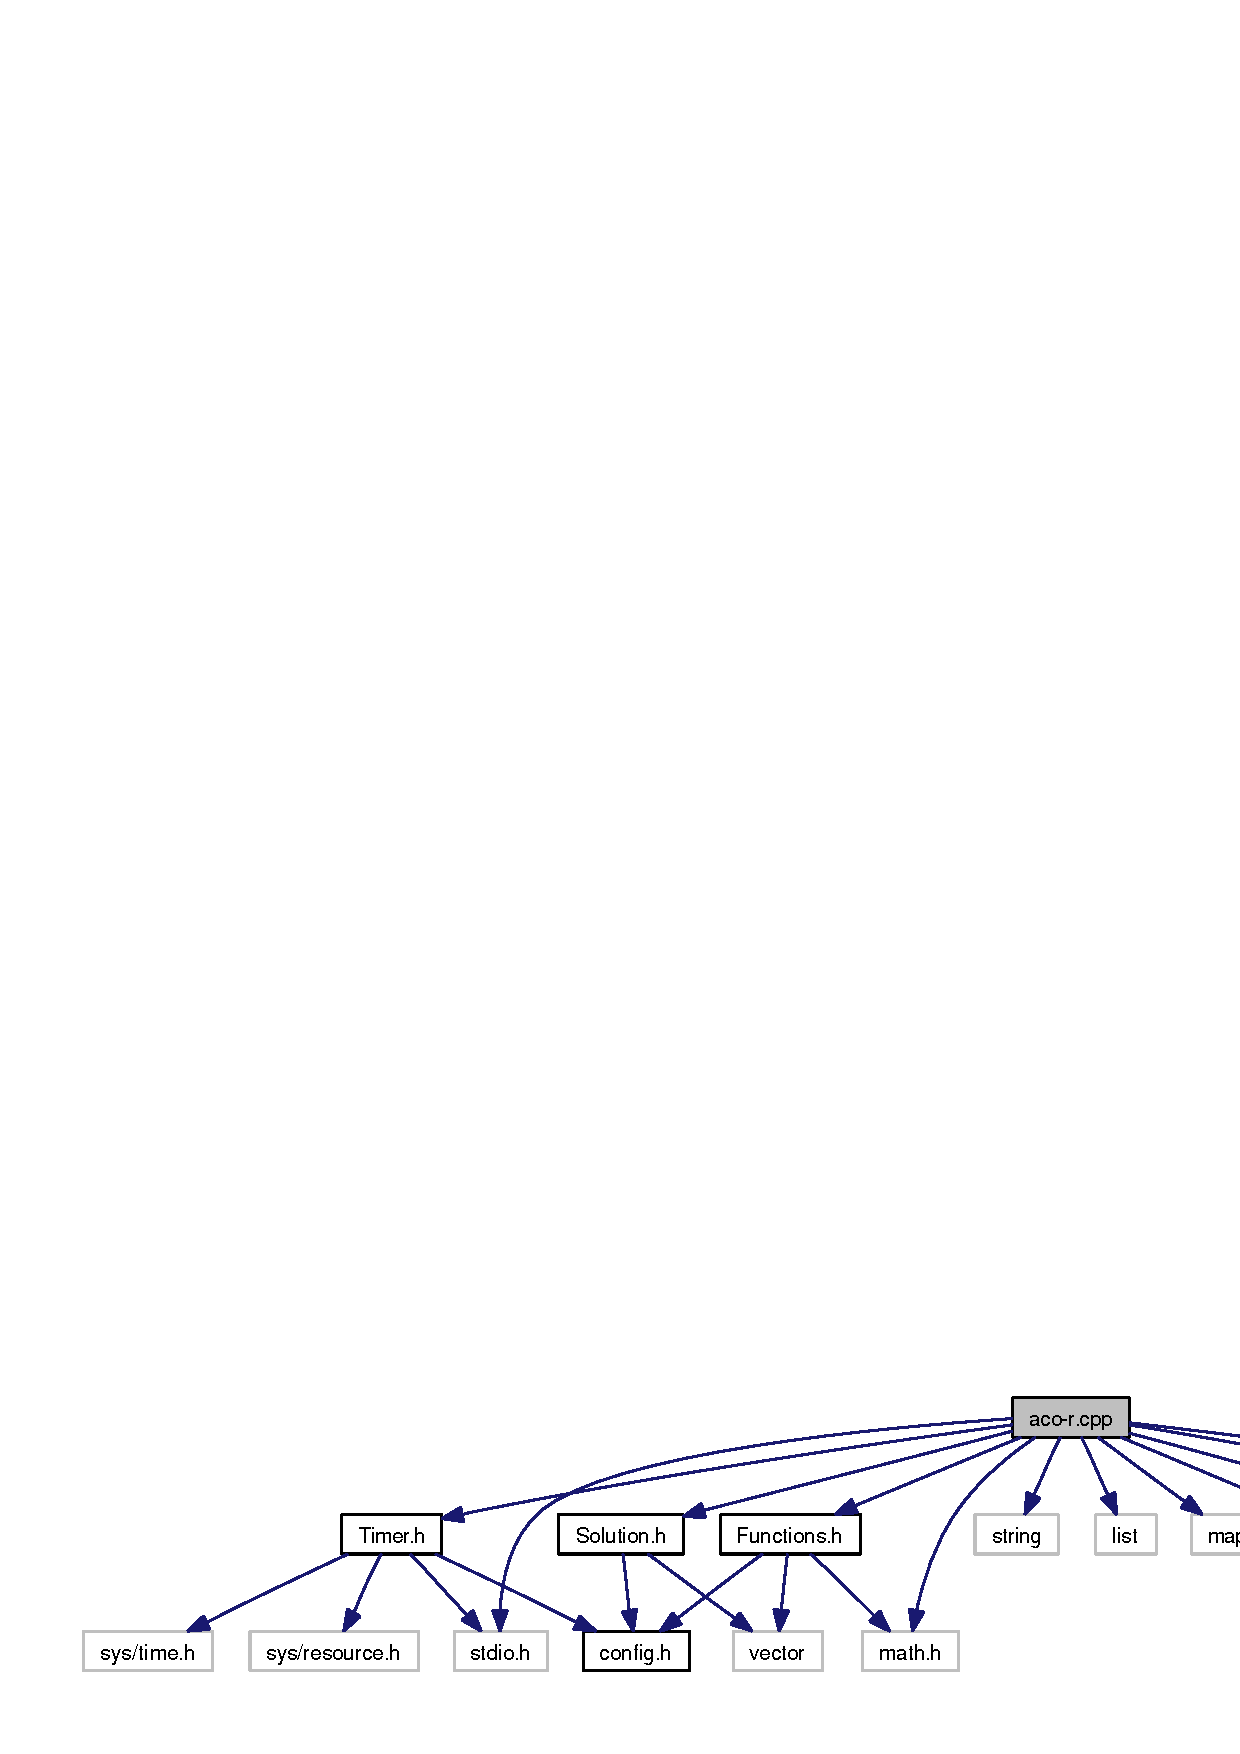
\includegraphics[width=420pt]{aco-r_8cpp__incl}
\end{center}
\end{figure}
\subsection*{Defines}
\begin{CompactItemize}
\item 
\#define \hyperlink{aco-r_8cpp_523b1c70fbff9e4e25f29b323bead209}{RAND\_\-UNIFORME}~(double)random()/(double)RAND\_\-MAX
\end{CompactItemize}
\subsection*{Functions}
\begin{CompactItemize}
\item 
void \hyperlink{aco-r_8cpp_02fd73d861ef2e4aabb38c0c9ff82947}{init} ()
\item 
double \hyperlink{aco-r_8cpp_c49c8f28940eb73a2d3c5d4f54a77acb}{gaussian} (double mean, double var)
\item 
void \hyperlink{aco-r_8cpp_cec77708e3d6f73a14c252e8747c11b1}{print\_\-best\_\-solution} (\hyperlink{classSolution}{Solution} bSol, \hyperlink{classFunction}{Function} $\ast$af, \hyperlink{classTimer}{Timer} \&atimer, int icount)
\item 
double \hyperlink{aco-r_8cpp_c5992296530c3f2c91fb35345606b029}{evaluate} (double $\ast$s)
\item 
int \hyperlink{aco-r_8cpp_3c04138a5bfe5d72780bb7e82a18e627}{main} (int argc, char $\ast$$\ast$argv)
\end{CompactItemize}
\subsection*{Variables}
\begin{CompactItemize}
\item 
double $\ast$ \hyperlink{aco-r_8cpp_a0e91b6673e0f6c62ed362a35d18064e}{archive} = NULL
\item 
double $\ast$ \hyperlink{aco-r_8cpp_68e32a83dbc9e45c0eca86384c297aba}{constrains} = NULL
\item 
int \hyperlink{aco-r_8cpp_1a8a8235879363159315091a1daed72f}{dimension} = 10
\item 
int \hyperlink{aco-r_8cpp_ae8c272782ff802dd95092adf15f474e}{archive\_\-size} = 5
\item 
int \hyperlink{aco-r_8cpp_346cfde20df32ef1244e37b7de85f5a3}{number\_\-of\_\-ants} = 3
\item 
int \hyperlink{aco-r_8cpp_77d5d27d8fdf89eb369e3bae9e6e752d}{number\_\-of\_\-iterations} = 100
\item 
double \hyperlink{aco-r_8cpp_5b5e3f03e443adea974601f295136638}{q} = 1.0
\item 
double \hyperlink{aco-r_8cpp_3ed57096651b587c2bf716fa78048153}{rho} = 1.0
\end{CompactItemize}


\subsection{Define Documentation}
\hypertarget{aco-r_8cpp_523b1c70fbff9e4e25f29b323bead209}{
\index{aco-r.cpp@{aco-r.cpp}!RAND\_\-UNIFORME@{RAND\_\-UNIFORME}}
\index{RAND\_\-UNIFORME@{RAND\_\-UNIFORME}!aco-r.cpp@{aco-r.cpp}}
\subsubsection{\setlength{\rightskip}{0pt plus 5cm}\#define RAND\_\-UNIFORME~(double)random()/(double)RAND\_\-MAX}}
\label{aco-r_8cpp_523b1c70fbff9e4e25f29b323bead209}




\subsection{Function Documentation}
\hypertarget{aco-r_8cpp_c5992296530c3f2c91fb35345606b029}{
\index{aco-r.cpp@{aco-r.cpp}!evaluate@{evaluate}}
\index{evaluate@{evaluate}!aco-r.cpp@{aco-r.cpp}}
\subsubsection{\setlength{\rightskip}{0pt plus 5cm}double evaluate (double $\ast$ {\em s})}}
\label{aco-r_8cpp_c5992296530c3f2c91fb35345606b029}


\hypertarget{aco-r_8cpp_c49c8f28940eb73a2d3c5d4f54a77acb}{
\index{aco-r.cpp@{aco-r.cpp}!gaussian@{gaussian}}
\index{gaussian@{gaussian}!aco-r.cpp@{aco-r.cpp}}
\subsubsection{\setlength{\rightskip}{0pt plus 5cm}double gaussian (double {\em mean}, \/  double {\em var})}}
\label{aco-r_8cpp_c49c8f28940eb73a2d3c5d4f54a77acb}


\hypertarget{aco-r_8cpp_02fd73d861ef2e4aabb38c0c9ff82947}{
\index{aco-r.cpp@{aco-r.cpp}!init@{init}}
\index{init@{init}!aco-r.cpp@{aco-r.cpp}}
\subsubsection{\setlength{\rightskip}{0pt plus 5cm}void init ()}}
\label{aco-r_8cpp_02fd73d861ef2e4aabb38c0c9ff82947}


\hypertarget{aco-r_8cpp_3c04138a5bfe5d72780bb7e82a18e627}{
\index{aco-r.cpp@{aco-r.cpp}!main@{main}}
\index{main@{main}!aco-r.cpp@{aco-r.cpp}}
\subsubsection{\setlength{\rightskip}{0pt plus 5cm}int main (int {\em argc}, \/  char $\ast$$\ast$ {\em argv})}}
\label{aco-r_8cpp_3c04138a5bfe5d72780bb7e82a18e627}




Here is the call graph for this function:\nopagebreak
\begin{figure}[H]
\begin{center}
\leavevmode
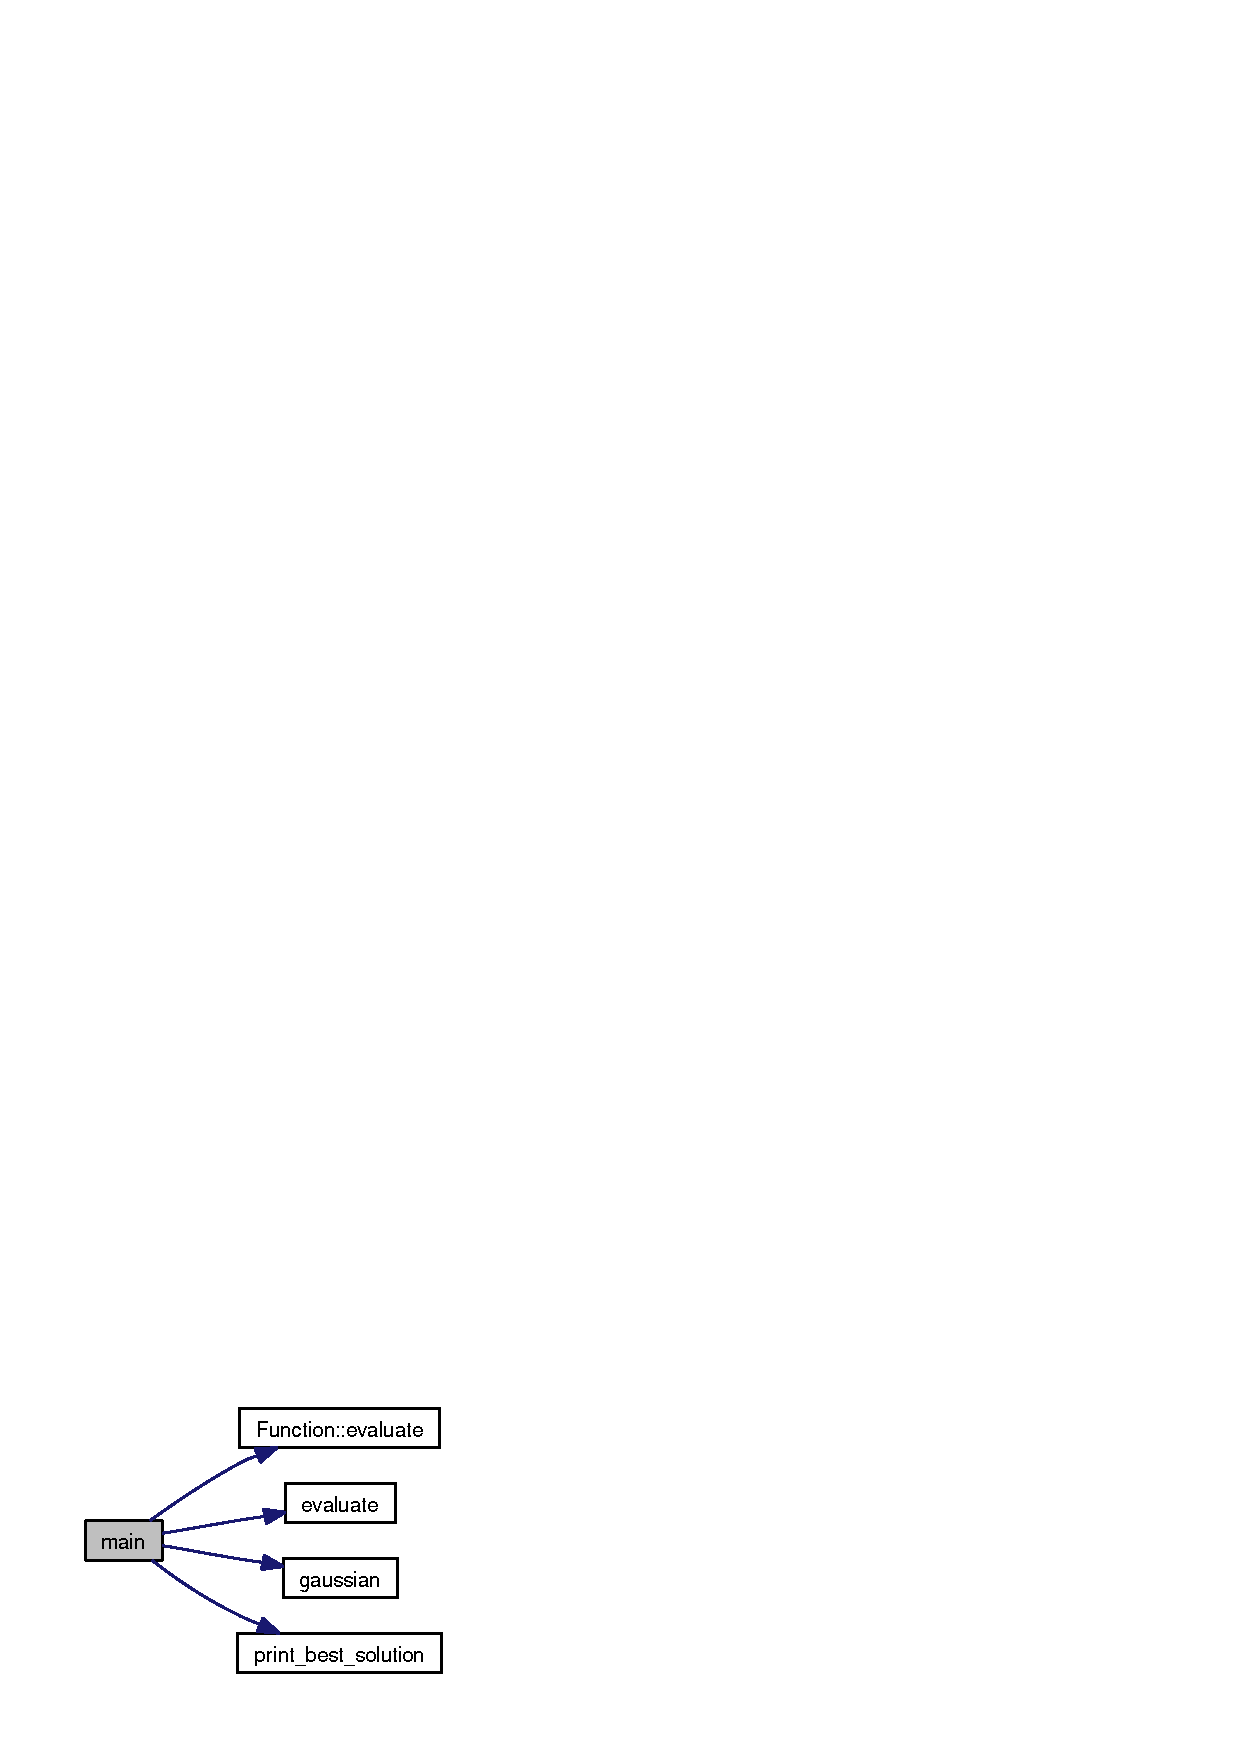
\includegraphics[width=108pt]{aco-r_8cpp_3c04138a5bfe5d72780bb7e82a18e627_cgraph}
\end{center}
\end{figure}
\hypertarget{aco-r_8cpp_cec77708e3d6f73a14c252e8747c11b1}{
\index{aco-r.cpp@{aco-r.cpp}!print\_\-best\_\-solution@{print\_\-best\_\-solution}}
\index{print\_\-best\_\-solution@{print\_\-best\_\-solution}!aco-r.cpp@{aco-r.cpp}}
\subsubsection{\setlength{\rightskip}{0pt plus 5cm}void print\_\-best\_\-solution ({\bf Solution} {\em bSol}, \/  {\bf Function} $\ast$ {\em af}, \/  {\bf Timer} \& {\em atimer}, \/  int {\em icount})}}
\label{aco-r_8cpp_cec77708e3d6f73a14c252e8747c11b1}




\subsection{Variable Documentation}
\hypertarget{aco-r_8cpp_a0e91b6673e0f6c62ed362a35d18064e}{
\index{aco-r.cpp@{aco-r.cpp}!archive@{archive}}
\index{archive@{archive}!aco-r.cpp@{aco-r.cpp}}
\subsubsection{\setlength{\rightskip}{0pt plus 5cm}double$\ast$ {\bf archive} = NULL}}
\label{aco-r_8cpp_a0e91b6673e0f6c62ed362a35d18064e}


\hypertarget{aco-r_8cpp_ae8c272782ff802dd95092adf15f474e}{
\index{aco-r.cpp@{aco-r.cpp}!archive\_\-size@{archive\_\-size}}
\index{archive\_\-size@{archive\_\-size}!aco-r.cpp@{aco-r.cpp}}
\subsubsection{\setlength{\rightskip}{0pt plus 5cm}int {\bf archive\_\-size} = 5}}
\label{aco-r_8cpp_ae8c272782ff802dd95092adf15f474e}


\hypertarget{aco-r_8cpp_68e32a83dbc9e45c0eca86384c297aba}{
\index{aco-r.cpp@{aco-r.cpp}!constrains@{constrains}}
\index{constrains@{constrains}!aco-r.cpp@{aco-r.cpp}}
\subsubsection{\setlength{\rightskip}{0pt plus 5cm}double$\ast$ {\bf constrains} = NULL}}
\label{aco-r_8cpp_68e32a83dbc9e45c0eca86384c297aba}


\hypertarget{aco-r_8cpp_1a8a8235879363159315091a1daed72f}{
\index{aco-r.cpp@{aco-r.cpp}!dimension@{dimension}}
\index{dimension@{dimension}!aco-r.cpp@{aco-r.cpp}}
\subsubsection{\setlength{\rightskip}{0pt plus 5cm}int {\bf dimension} = 10}}
\label{aco-r_8cpp_1a8a8235879363159315091a1daed72f}


\hypertarget{aco-r_8cpp_346cfde20df32ef1244e37b7de85f5a3}{
\index{aco-r.cpp@{aco-r.cpp}!number\_\-of\_\-ants@{number\_\-of\_\-ants}}
\index{number\_\-of\_\-ants@{number\_\-of\_\-ants}!aco-r.cpp@{aco-r.cpp}}
\subsubsection{\setlength{\rightskip}{0pt plus 5cm}int {\bf number\_\-of\_\-ants} = 3}}
\label{aco-r_8cpp_346cfde20df32ef1244e37b7de85f5a3}


\hypertarget{aco-r_8cpp_77d5d27d8fdf89eb369e3bae9e6e752d}{
\index{aco-r.cpp@{aco-r.cpp}!number\_\-of\_\-iterations@{number\_\-of\_\-iterations}}
\index{number\_\-of\_\-iterations@{number\_\-of\_\-iterations}!aco-r.cpp@{aco-r.cpp}}
\subsubsection{\setlength{\rightskip}{0pt plus 5cm}int {\bf number\_\-of\_\-iterations} = 100}}
\label{aco-r_8cpp_77d5d27d8fdf89eb369e3bae9e6e752d}


\hypertarget{aco-r_8cpp_5b5e3f03e443adea974601f295136638}{
\index{aco-r.cpp@{aco-r.cpp}!q@{q}}
\index{q@{q}!aco-r.cpp@{aco-r.cpp}}
\subsubsection{\setlength{\rightskip}{0pt plus 5cm}double {\bf q} = 1.0}}
\label{aco-r_8cpp_5b5e3f03e443adea974601f295136638}


\hypertarget{aco-r_8cpp_3ed57096651b587c2bf716fa78048153}{
\index{aco-r.cpp@{aco-r.cpp}!rho@{rho}}
\index{rho@{rho}!aco-r.cpp@{aco-r.cpp}}
\subsubsection{\setlength{\rightskip}{0pt plus 5cm}double {\bf rho} = 1.0}}
\label{aco-r_8cpp_3ed57096651b587c2bf716fa78048153}



\hypertarget{Colony_8cpp}{
\section{Colony.cpp File Reference}
\label{Colony_8cpp}\index{Colony.cpp@{Colony.cpp}}
}
{\tt \#include $<$iostream$>$}\par
{\tt \#include $<$fstream$>$}\par
{\tt \#include $<$stdio.h$>$}\par
{\tt \#include \char`\"{}Colony.h\char`\"{}}\par


Include dependency graph for Colony.cpp:\nopagebreak
\begin{figure}[H]
\begin{center}
\leavevmode
\includegraphics[width=220pt]{Colony_8cpp__incl}
\end{center}
\end{figure}

\hypertarget{Colony_8h}{
\section{Colony.h File Reference}
\label{Colony_8h}\index{Colony.h@{Colony.h}}
}
{\tt \#include \char`\"{}config.h\char`\"{}}\par
{\tt \#include $<$vector$>$}\par
{\tt \#include $<$map$>$}\par
{\tt \#include $<$list$>$}\par
{\tt \#include $<$cstdlib$>$}\par
{\tt \#include \char`\"{}Solution.h\char`\"{}}\par
{\tt \#include \char`\"{}Functions.h\char`\"{}}\par


Include dependency graph for Colony.h:\nopagebreak
\begin{figure}[H]
\begin{center}
\leavevmode
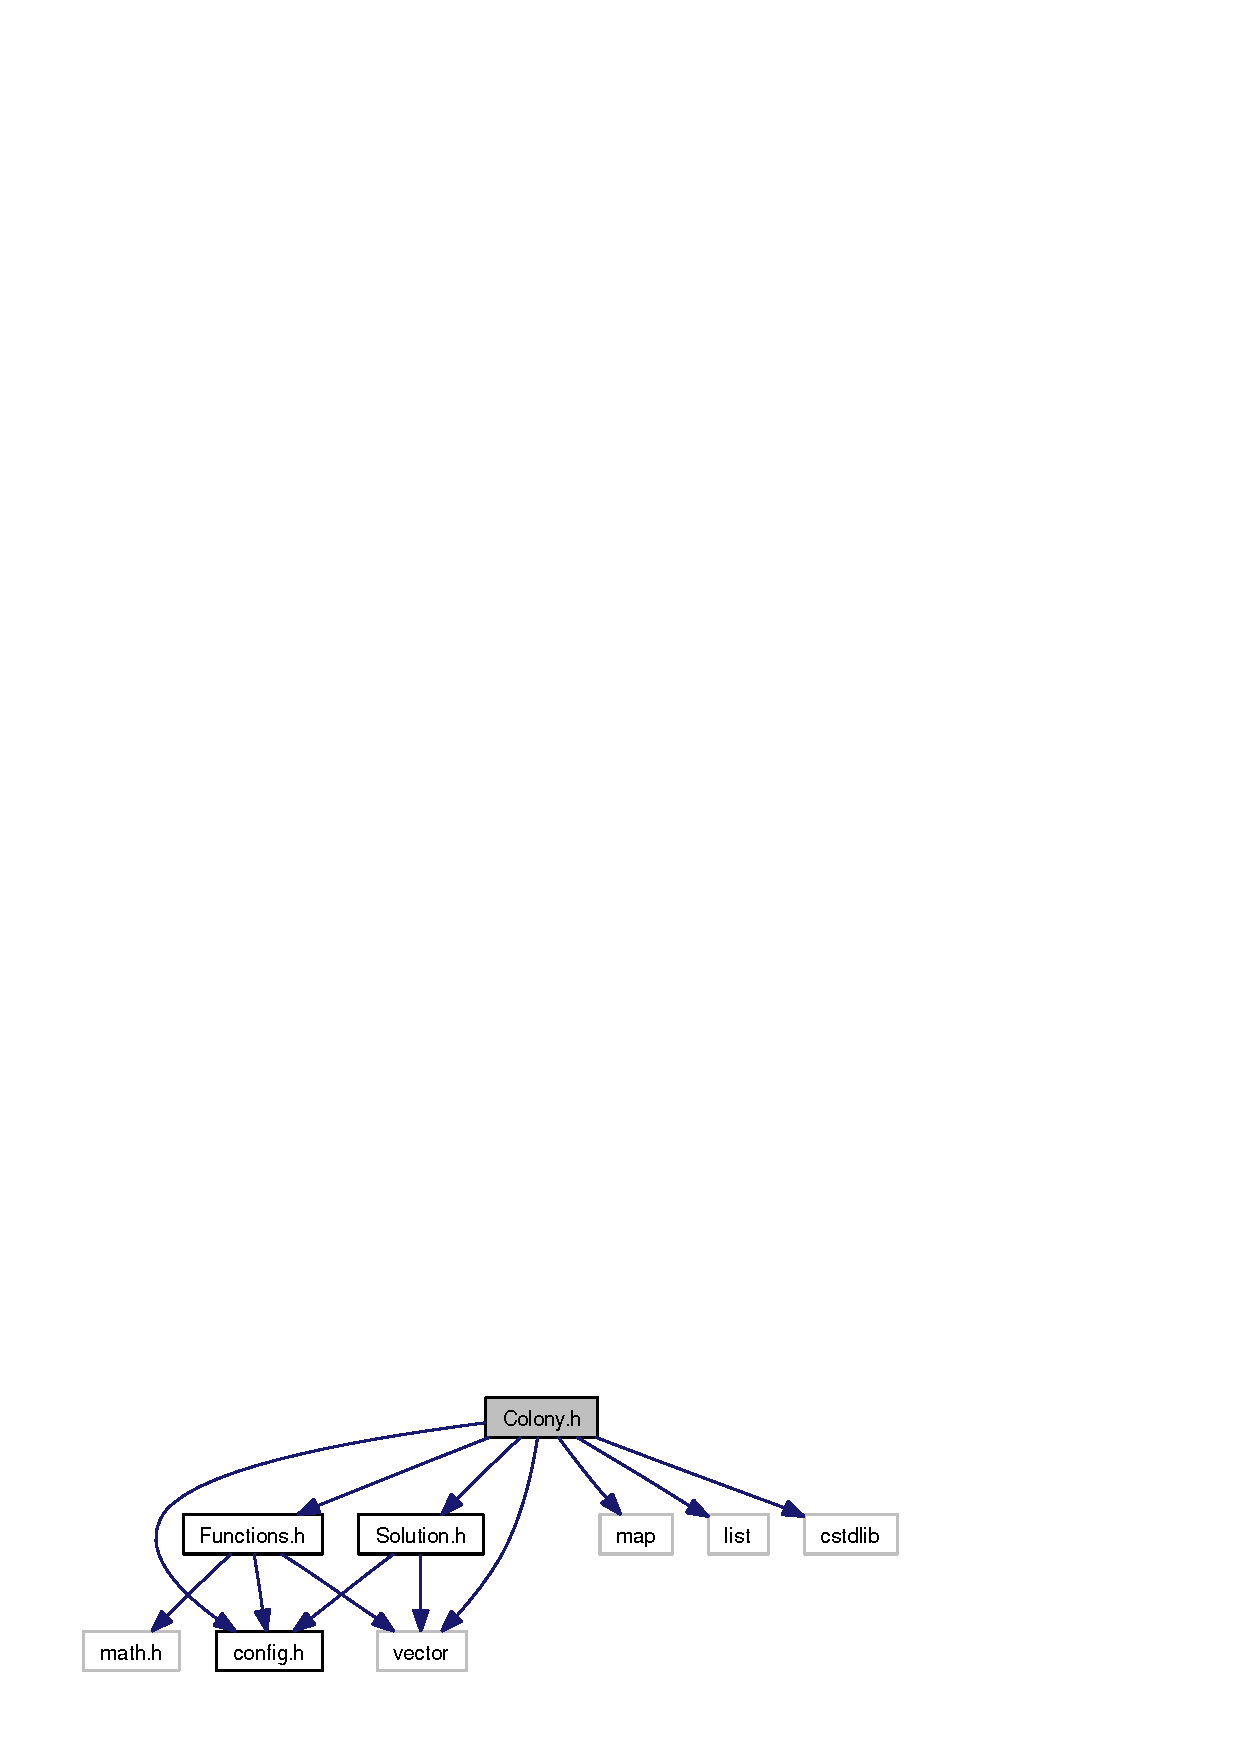
\includegraphics[width=217pt]{Colony_8h__incl}
\end{center}
\end{figure}


This graph shows which files directly or indirectly include this file:\nopagebreak
\begin{figure}[H]
\begin{center}
\leavevmode
\includegraphics[width=54pt]{Colony_8h__dep__incl}
\end{center}
\end{figure}
\subsection*{Classes}
\begin{CompactItemize}
\item 
class \hyperlink{classColony}{Colony}
\end{CompactItemize}

\hypertarget{config_8h}{
\section{config.h File Reference}
\label{config_8h}\index{config.h@{config.h}}
}


This graph shows which files directly or indirectly include this file:\nopagebreak
\begin{figure}[H]
\begin{center}
\leavevmode
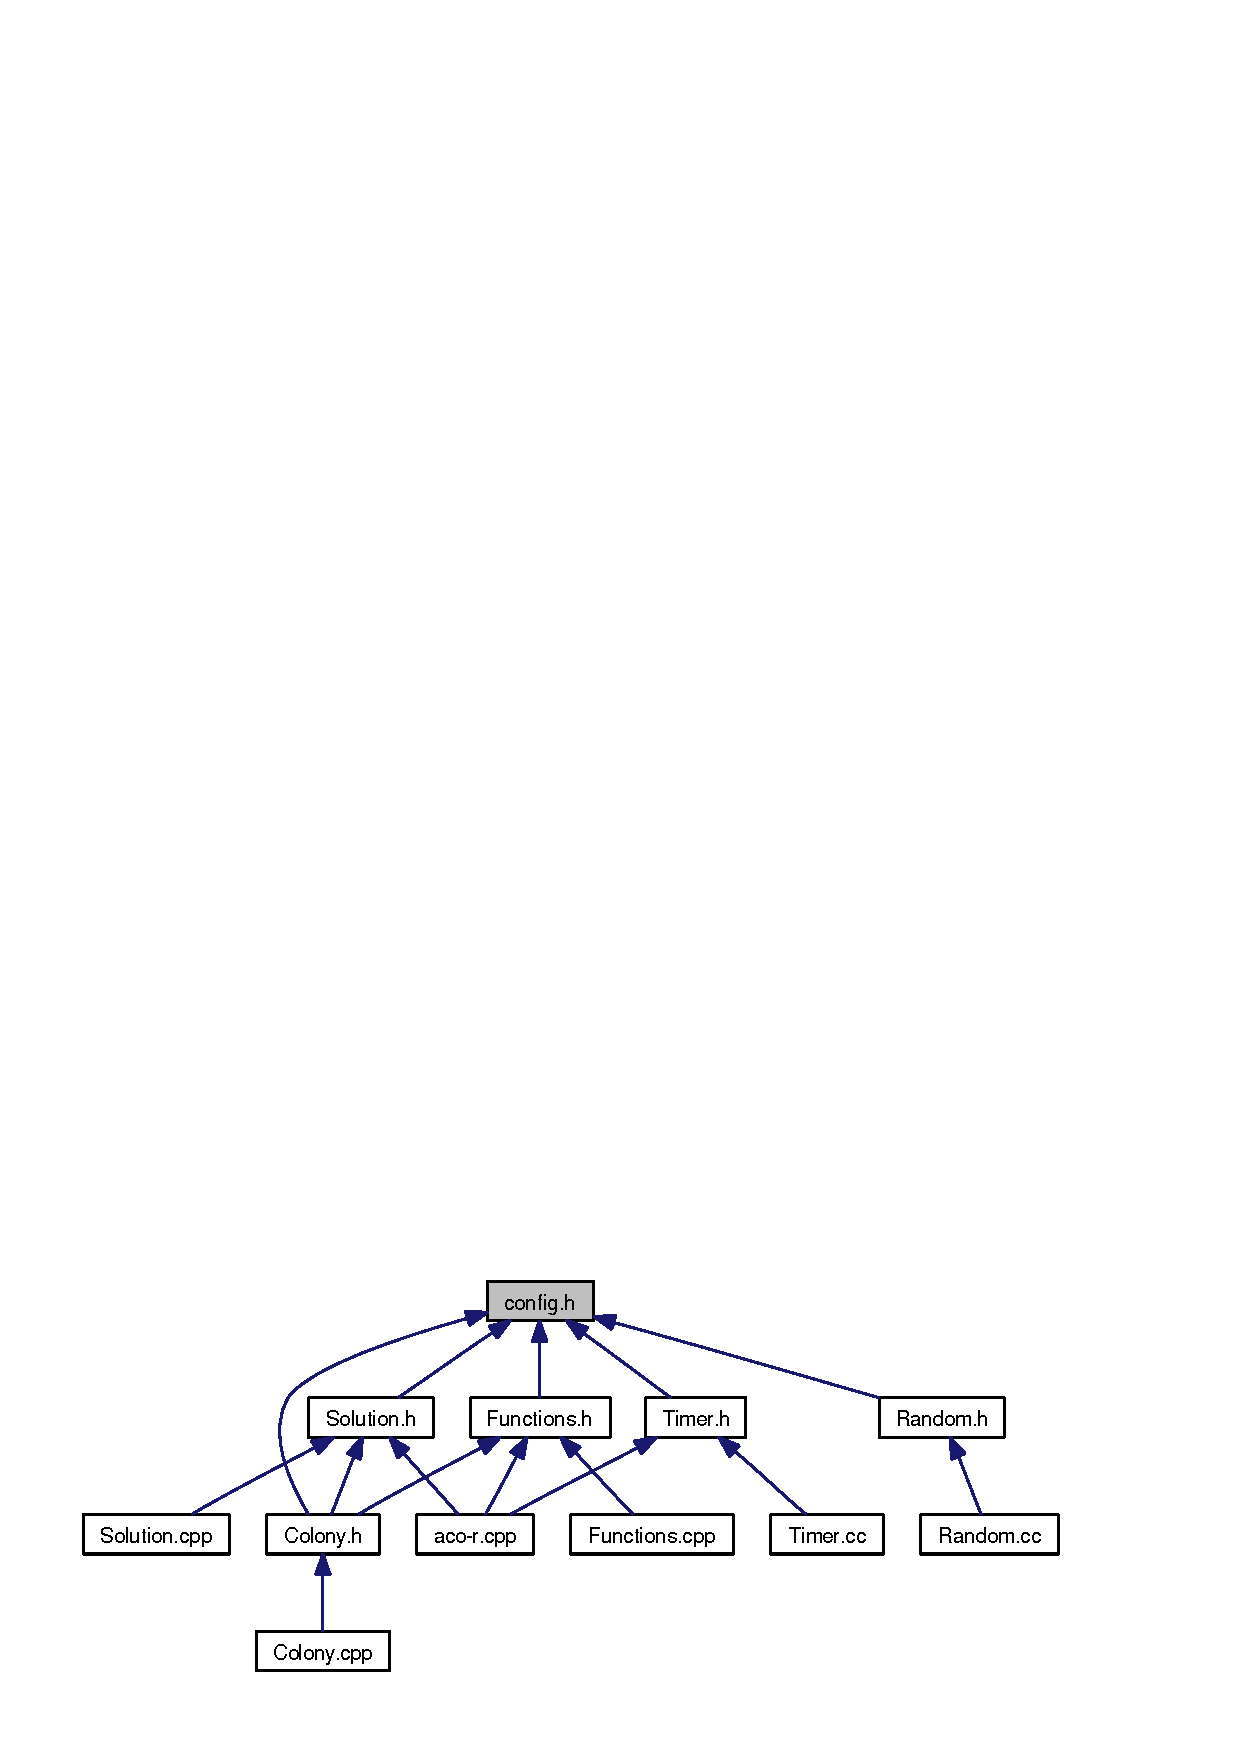
\includegraphics[width=256pt]{config_8h__dep__incl}
\end{center}
\end{figure}

\hypertarget{Functions_8cpp}{
\section{Functions.cpp File Reference}
\label{Functions_8cpp}\index{Functions.cpp@{Functions.cpp}}
}
{\tt \#include \char`\"{}Functions.h\char`\"{}}\par


Include dependency graph for Functions.cpp:\nopagebreak
\begin{figure}[H]
\begin{center}
\leavevmode
\includegraphics[width=109pt]{Functions_8cpp__incl}
\end{center}
\end{figure}

\hypertarget{Functions_8h}{
\section{Functions.h File Reference}
\label{Functions_8h}\index{Functions.h@{Functions.h}}
}
{\tt \#include \char`\"{}config.h\char`\"{}}\par
{\tt \#include $<$vector$>$}\par
{\tt \#include $<$math.h$>$}\par


Include dependency graph for Functions.h:\nopagebreak
\begin{figure}[H]
\begin{center}
\leavevmode
\includegraphics[width=109pt]{Functions_8h__incl}
\end{center}
\end{figure}


This graph shows which files directly or indirectly include this file:\nopagebreak
\begin{figure}[H]
\begin{center}
\leavevmode
\includegraphics[width=134pt]{Functions_8h__dep__incl}
\end{center}
\end{figure}
\subsection*{Classes}
\begin{CompactItemize}
\item 
class \hyperlink{classFunction}{Function}
\item 
class \hyperlink{classGriewank}{Griewank}
\item 
class \hyperlink{classAckley}{Ackley}
\item 
class \hyperlink{classRastrigin}{Rastrigin}
\end{CompactItemize}

\hypertarget{Random_8cc}{
\section{Random.cc File Reference}
\label{Random_8cc}\index{Random.cc@{Random.cc}}
}
{\tt \#include \char`\"{}Random.h\char`\"{}}\par
{\tt \#include $<$stdio.h$>$}\par


Include dependency graph for Random.cc:\nopagebreak
\begin{figure}[H]
\begin{center}
\leavevmode
\includegraphics[width=147pt]{Random_8cc__incl}
\end{center}
\end{figure}
\subsection*{Defines}
\begin{CompactItemize}
\item 
\#define \hyperlink{Random_8cc_ce2e8e5cd08b605ab70bbf1a81185972}{VERBOSE}(x)~x
\item 
\#define \hyperlink{Random_8cc_61bdcb2fd2ebb805a31bde1ce782d732}{VERYVERBOSE}(x)
\end{CompactItemize}


\subsection{Define Documentation}
\hypertarget{Random_8cc_ce2e8e5cd08b605ab70bbf1a81185972}{
\index{Random.cc@{Random.cc}!VERBOSE@{VERBOSE}}
\index{VERBOSE@{VERBOSE}!Random.cc@{Random.cc}}
\subsubsection{\setlength{\rightskip}{0pt plus 5cm}\#define VERBOSE(x)~x}}
\label{Random_8cc_ce2e8e5cd08b605ab70bbf1a81185972}


\hypertarget{Random_8cc_61bdcb2fd2ebb805a31bde1ce782d732}{
\index{Random.cc@{Random.cc}!VERYVERBOSE@{VERYVERBOSE}}
\index{VERYVERBOSE@{VERYVERBOSE}!Random.cc@{Random.cc}}
\subsubsection{\setlength{\rightskip}{0pt plus 5cm}\#define VERYVERBOSE(x)}}
\label{Random_8cc_61bdcb2fd2ebb805a31bde1ce782d732}



\hypertarget{Random_8h}{
\section{Random.h File Reference}
\label{Random_8h}\index{Random.h@{Random.h}}
}
{\tt \#include \char`\"{}config.h\char`\"{}}\par
{\tt \#include $<$algorithm$>$}\par
{\tt \#include $<$vector$>$}\par
{\tt \#include $<$stdlib.h$>$}\par


Include dependency graph for Random.h:\nopagebreak
\begin{figure}[H]
\begin{center}
\leavevmode
\includegraphics[width=147pt]{Random_8h__incl}
\end{center}
\end{figure}


This graph shows which files directly or indirectly include this file:\nopagebreak
\begin{figure}[H]
\begin{center}
\leavevmode
\includegraphics[width=55pt]{Random_8h__dep__incl}
\end{center}
\end{figure}
\subsection*{Classes}
\begin{CompactItemize}
\item 
class \hyperlink{classRandom}{Random}
\end{CompactItemize}

\hypertarget{Solution_8cpp}{
\section{Solution.cpp File Reference}
\label{Solution_8cpp}\index{Solution.cpp@{Solution.cpp}}
}
{\tt \#include \char`\"{}Solution.h\char`\"{}}\par


Include dependency graph for Solution.cpp:\nopagebreak
\begin{figure}[H]
\begin{center}
\leavevmode
\includegraphics[width=77pt]{Solution_8cpp__incl}
\end{center}
\end{figure}

\hypertarget{Solution_8h}{
\section{Solution.h File Reference}
\label{Solution_8h}\index{Solution.h@{Solution.h}}
}
{\tt \#include \char`\"{}config.h\char`\"{}}\par
{\tt \#include $<$vector$>$}\par


Include dependency graph for Solution.h:\nopagebreak
\begin{figure}[H]
\begin{center}
\leavevmode
\includegraphics[width=77pt]{Solution_8h__incl}
\end{center}
\end{figure}


This graph shows which files directly or indirectly include this file:\nopagebreak
\begin{figure}[H]
\begin{center}
\leavevmode
\includegraphics[width=130pt]{Solution_8h__dep__incl}
\end{center}
\end{figure}
\subsection*{Classes}
\begin{CompactItemize}
\item 
class \hyperlink{classSolution}{Solution}
\end{CompactItemize}

\hypertarget{Timer_8cc}{
\section{Timer.cc File Reference}
\label{Timer_8cc}\index{Timer.cc@{Timer.cc}}
}
{\tt \#include \char`\"{}Timer.h\char`\"{}}\par


Include dependency graph for Timer.cc:\nopagebreak
\begin{figure}[H]
\begin{center}
\leavevmode
\includegraphics[width=167pt]{Timer_8cc__incl}
\end{center}
\end{figure}

\hypertarget{Timer_8h}{
\section{Timer.h File Reference}
\label{Timer_8h}\index{Timer.h@{Timer.h}}
}
{\tt \#include \char`\"{}config.h\char`\"{}}\par
{\tt \#include $<$sys/time.h$>$}\par
{\tt \#include $<$sys/resource.h$>$}\par
{\tt \#include $<$stdio.h$>$}\par


Include dependency graph for Timer.h:\nopagebreak
\begin{figure}[H]
\begin{center}
\leavevmode
\includegraphics[width=167pt]{Timer_8h__incl}
\end{center}
\end{figure}


This graph shows which files directly or indirectly include this file:\nopagebreak
\begin{figure}[H]
\begin{center}
\leavevmode
\includegraphics[width=86pt]{Timer_8h__dep__incl}
\end{center}
\end{figure}
\subsection*{Classes}
\begin{CompactItemize}
\item 
class \hyperlink{classTimer}{Timer}
\end{CompactItemize}

\printindex
\end{document}
